%%%%%%%%%%%%%%%%%%%%%%%%%%%%%%%%%%%%%%%%%%%%%%%%%%%%%%%%%%%%%%%%%%%%%%%
%  ENVIO MULTILINGUE (arXiv, politica vigente desde 11/02/2026)
%  Version inglesa primero, version castellana despues.
%
%  The Holographic Theory of State Persistence confronted with
%  DESI DR2, Pantheon+ and the CMB
%
%  Moises Mora Garcia & Jorge Ordonez Mora
%  Palma de Mallorca, Spain -- 2026
%
%  Compile with:  pdflatex THPE_arxiv_EN.tex   (twice, for references)
%  Requires: revtex4-2 (standard in TeX Live / MiKTeX)
%
%  NOTE FOR THE AUTHORS: figures THPE_v18_dr2_resultados.png and
%  THPE_v18_dr2_corner.png must be in the same folder as this file.
%  If they are absent the document still compiles (figures are wrapped
%  in \IfFileExists), but the figure slots will be empty.
%%%%%%%%%%%%%%%%%%%%%%%%%%%%%%%%%%%%%%%%%%%%%%%%%%%%%%%%%%%%%%%%%%%%%%%

\documentclass[aps,prd,twocolumn,superscriptaddress,nofootinbib,floatfix]{revtex4-2}

\usepackage{amsmath,amssymb}
\usepackage{graphicx}
\usepackage{hyperref}
\hypersetup{colorlinks=true,linkcolor=blue,citecolor=blue,urlcolor=blue}
\usepackage[utf8]{inputenc}

\newcommand{\LCDM}{\ensuremath{\Lambda}CDM}
\newcommand{\Msun}{M_\odot}

\begin{document}

\title{The Holographic Theory of State Persistence confronted with
DESI DR2, Pantheon+ and the CMB: observational bounds and theoretical
localisation of an informational extension of holographic dark energy}

\author{Mois\'es Mora Garc\'ia}
\affiliation{Independent researcher, Palma de Mallorca, Spain}
\author{Jorge Ord\'o\~nez Mora}
\affiliation{Independent researcher, Palma de Mallorca, Spain}

\date{\today}

\begin{abstract}
We present the Holographic Theory of State Persistence (THPE), a
phenomenological extension of holographic dark energy in which the dark
energy density is promoted to a field
$\Phi(z)=\Phi_0[1+\alpha f_{\rm SFR}(z)+\beta g_{\rm struct}(z)+\gamma
h_{\rm ent}(z)]$ tied to three tracers of informational complexity:
star formation, large-scale structure and horizon entropy. The model
recovers \LCDM{} exactly for $\alpha=\beta=\gamma=0$ and predicts a
crossing of $w(z)=-1$ synchronised with the star formation history.
We report two complementary results. (i) Confronting the model with
DESI DR2 baryon acoustic oscillations (13 measurements with per-tracer
correlations), the Pantheon+ Type~Ia supernova compilation (1588
objects with the full statistical-plus-systematic covariance and the
absolute calibration analytically marginalised) and the compressed CMB
distance priors from Planck 2018, nested sampling yields
$\ln B=-7.4\pm0.2$ in favour of \LCDM{} against the minimal
single-tracer variant and $\ln B=-14.8\pm0.2$ against the
three-parameter variant: strong evidence on the Jeffreys scale in all
cases. The horizon-entropy term is excluded by physicality
($|\gamma|\lesssim10^{-3}$) and the final bounds are $\alpha<0.008$ and
$\beta<0.07$ (68\% CL), so that any informational contribution to the
holographic pressure lies below $\sim1\%$ of the dark energy density.
(ii) Investigating whether $\Phi(z)$ can be derived rather than
postulated, we find that a covariant action with non-minimal coupling
does generate $\Box\Pi=I$ with the source fixed by the coupling, and
that the construction passes ghost, degrees-of-freedom and
conservation tests; however, the Cassini bound on the scalar sector is
$\sim400$ times more restrictive than cosmology, and the known
screening mechanisms lead to theories already present in the
literature. We conclude that the local scalar--tensor formulation of
the THPE provides no independent phenomenological content relative to
the Horndeski theories surviving GW170817. We additionally show that
identifying the Compton time $\tau_c=\hbar/Mc^2$ as a universal
state-compression rate is refuted by demonstrated quantum coherence by
14 to 51 orders of magnitude. The full pipeline, its coherence
controls and the complete correction history are made public. The
prediction of a $w=-1$ crossing tied to star formation remains
registered as a falsifiable test for the coming decade.
\vskip4pt
\noindent\emph{Note on languages:} this is a multilingual submission.
The English version appears first; a full Spanish translation follows
(original language of composition: Spanish). In case of discrepancy the
English version prevails.
\end{abstract}

\maketitle

%=======================================================================
\section{Introduction}
%=======================================================================

The nature of dark energy remains unexplained. Recent DESI results have
reopened the possibility that its equation of state evolves with time
\cite{DESI2024,DESI2025}, motivating the study of dynamical extensions
of \LCDM{}.

The THPE proposes one such extension: that the dark energy density be
tied to the informational content of the universe --- the complexity
generated by star formation, structure growth and horizon entropy. The
underlying motivation is that a universe which produces structure might
leave a measurable imprint on its own expansion.

This paper does not defend that hypothesis: it tests it. An earlier
version of this work presented the model as a proposal with qualitative
compatibility. The present version reports the complete outcome of two
consecutive research programmes --- one observational and one
mathematical --- both with acceptance criteria fixed in advance, and
both yielding negative results which we publish in full. We regard the
delimitation of the viable parameter space of a hypothesis as a
legitimate scientific product.

The paper is organised as follows. Section~\ref{sec:theory} presents
the model. Section~\ref{sec:data} describes the data and the inference
methodology, including the coherence controls. Section~\ref{sec:results}
reports the observational results. Section~\ref{sec:compton} refutes the
local Compton scale. Section~\ref{sec:derivation} reports the attempt to
derive $\Phi(z)$ from an action principle and localises the resulting
theory. Sections~\ref{sec:discussion}--\ref{sec:future} discuss the
limitations and the future testability of the prediction.

%=======================================================================
\section{Theoretical framework}
\label{sec:theory}
%=======================================================================

\subsection{Formulation}

The THPE promotes the dark energy density to
%
\begin{equation}
\Phi(z)=\Phi_0\left[1+\alpha f_{\rm SFR}(z)+\beta g_{\rm struct}(z)
+\gamma h_{\rm ent}(z)\right],
\label{eq:phi}
\end{equation}
%
where $f_{\rm SFR}$ is the normalised cosmic star formation rate
\cite{Madau2014}, $g_{\rm struct}$ a normalised large-scale structure
density, and $h_{\rm ent}$ the horizon entropy per comoving volume.
The Friedmann equation reads
%
\begin{equation}
H^2(z)=H_0^2\left[\Omega_m(1+z)^3+\Omega_r(1+z)^4+\Phi(z)\right],
\label{eq:friedmann}
\end{equation}
%
and the effective equation of state is
%
\begin{equation}
w(z)=-1+\frac{1+z}{3\,\Phi}\frac{d\Phi}{dz}.
\label{eq:woz}
\end{equation}
%
For $\alpha=\beta=\gamma=0$, Eq.~(\ref{eq:phi}) gives $\Phi=\Phi_0$ and
\LCDM{} is recovered exactly, with $\Phi_0=\Omega_\Lambda$. The
characteristic prediction is a crossing of $w(z)=-1$ whose chronology
follows the peak of star formation at $z\simeq1.9$.

\subsection{Relation to previous work}

The Hilbert-space layer structure separated by the Planck time
coincides with the Holographic Space-Time framework of Banks and
Fischler \cite{Banks2011}; we state this without claiming originality on
that point. The proposed contribution was the explicit link between the
holographic pressure and observable tracers of complexity.
Section~\ref{sec:everpresent} documents a direct precedent for the
underlying intuition in the causal set literature.

\subsection{Status after this work}

Section~\ref{sec:derivation} shows that the local scalar--tensor version
of Eq.~(\ref{eq:phi}) is localised within an already studied space of
theories. Accordingly, Eq.~(\ref{eq:phi}) is to be understood in this
paper as an observationally bounded \emph{phenomenological
parametrisation}, not as a proposal of new fundamental physics.

%=======================================================================
\section{Data and methodology}
\label{sec:data}
%=======================================================================

\subsection{Data}

We use three datasets.

\emph{(i) DESI DR2 BAO} \cite{DESI2025}: 13 measurements ---
$D_V/r_d$ for the BGS tracer, and the pairs
$(D_M/r_d,\,D_H/r_d)$ with their correlation coefficients for LRG1,
LRG2, LRG3+ELG1, ELG2, QSO and Ly$\alpha$, spanning
$0.295\le z_{\rm eff}\le2.330$. The transcription of the data vector was
verified against two independent sources.

\emph{(ii) Pantheon+} \cite{Scolnic2022}: 1588 Type~Ia supernovae with
$z>0.01$ and the full statistical-plus-systematic covariance matrix.

\emph{(iii) Compressed CMB distance priors} from Planck 2018
\cite{Planck2020,Chen2019}: the shift parameter $R$ and the acoustic
scale $\ell_A$ with their correlation, self-calibrated to the fiducial
background of the pipeline. The common modelling offset ($\sim0.1\%$,
arising from the treatment of neutrinos and from the numerical
evaluation of $r_s$) is identical for all models and cancels by
construction; this choice is stated explicitly.

\subsection{Likelihoods}

For BAO we adopt a Gaussian likelihood with a block-diagonal covariance
per tracer. For supernovae we marginalise analytically over a constant
magnitude offset,
%
\begin{equation}
\chi^2_{\rm marg}=\Delta^{T}C^{-1}\Delta
-\frac{\left(\Delta^{T}C^{-1}\mathbf{1}\right)^2}
{\mathbf{1}^{T}C^{-1}\mathbf{1}},
\label{eq:marg}
\end{equation}
%
where $\Delta=\mu_{\rm obs}-\mu_{\rm th}$. This renders the result
independent of the SH0ES versus Planck absolute calibration. For the CMB
we use a two-dimensional Gaussian in $(R,\ell_A)$. The background is
fixed to Planck 2018 values ($H_0=67.4~{\rm km\,s^{-1}Mpc^{-1}}$,
$\Omega_m=0.315$); this limitation is discussed in
Sec.~\ref{sec:discussion}.

\subsection{Inference}

Priors: $\Phi_0$ log-uniform on $[10^{-3},2]$; $\alpha$ and $\beta$
uniform on $[0,10]$; $\gamma$ uniform on $[0,5]$ (negative values imply
$H^2<0$ at $z\lesssim0.01$, where supernovae exist, and are excluded
from the prior); $\Phi(z)>0$ is enforced on $0.011\le z\le4.5$.
Evidences are computed with nested sampling
(\textsc{dynesty} \cite{Speagle2020}, $n_{\rm live}=800$, slice
sampling).

We report a methodological warning of general applicability:
ensemble samplers of the Goodman--Weare type \cite{emcee} do
\emph{not} converge on this posterior. The extended
$\Phi_0$--$\alpha$--$\beta$ degeneracy produces Gelman--Rubin
statistics between 3 and 8 even with 64 walkers and 20000 steps.
Nested sampling converges and additionally provides the evidence.

\subsection{Coherence controls}
\label{sec:controls}

Two automatic controls were built into the pipeline.
\emph{(i) Reference-model coherence:} $\chi^2$ of \LCDM{} against each
data vector is computed at start-up, and execution aborts if it is
anomalous. \emph{(ii) Nesting condition:}
$\ln\mathcal{L}_{\rm max}({\rm THPE})\ge\ln\mathcal{L}_{\rm max}(\Lambda\mathrm{CDM})$
must hold, since the models are nested.

These controls detected and discarded three invalid results during the
campaign. The most instructive was a spurious $\ln B=+290$ \emph{in
favour} of the THPE, caused by a truncation in the numerical evaluation
of the sound horizon ($r_s=139.0$ instead of $144.4$~Mpc). We report
this explicitly because it illustrates that, in Bayesian model
comparison, a coherence control on the \emph{reference} model is
indispensable: an anomalous $\chi^2$ for the model known to work
signals a bookkeeping error, not a discovery.

%=======================================================================
\section{Observational results}
\label{sec:results}
%=======================================================================

\subsection{Evidences}

With the full geometric dataset (DESI DR2 BAO + Pantheon+ + CMB
distance priors) we obtain
%
\begin{align}
\Lambda\mathrm{CDM}~(1\,{\rm par.}) &: \quad \ln Z=-740.13\pm0.11,\nonumber\\
{\rm THPE}~\alpha{\rm -only}~(2\,{\rm par.}) &: \quad \ln Z=-747.56\pm0.16,\nonumber\\
{\rm THPE}~(\gamma=0,\;3\,{\rm par.}) &: \quad \ln Z=-754.92\pm0.19,
\end{align}
%
so that
%
\begin{align}
\ln B(\alpha\text{-only}/\Lambda\mathrm{CDM}) &= -7.43\pm0.19,\label{eq:lnB1}\\
\ln B(\text{3-par.}/\Lambda\mathrm{CDM}) &= -14.79\pm0.22.\label{eq:lnB2}
\end{align}
%
The nesting control is satisfied: the three models share
$\ln\mathcal{L}_{\rm max}=-733.50$. The best-fitting THPE configuration
coincides exactly with \LCDM{} ($\Delta\chi^2=0.0$). For \LCDM{} the
posterior gives $\Phi_0=0.6883$, consistent with the Planck value.

\subsection{Robustness chain}

The result is stable across dataset combinations:
%
\begin{center}
\begin{tabular}{lcc}
\hline\hline
Dataset & Statistic & Value \\
\hline
DR1 BAO+SNe (MCMC) & $\Delta{\rm AIC}$ & $+10.5$ \\
DR2 BAO+SNe & $\ln B$ (3-par.) & $-11.1$ \\
DR2 BAO+SNe & $\ln B$ ($\alpha$-only) & $-4.9$ \\
DR2+CMB & $\ln B$ (3-par.) & $-14.8$ \\
DR2+CMB & $\ln B$ ($\alpha$-only) & $-7.4$ \\
\hline\hline
\end{tabular}
\end{center}
%
Adding the CMB anchor \emph{worsens} the case for the THPE. Without the
anchor, \LCDM{} prefers $\Phi_0=0.724>0.685$, breaking flatness: the
mild ($\sim2.3\sigma$) DR2--Planck tension projects onto the
\emph{amplitude} of dark energy, not onto its functional form, and
neither $f_{\rm SFR}$ nor $g_{\rm struct}$ has the required shape.

\subsection{Parameter bounds}

At 68\% credibility,
%
\begin{equation}
\alpha<0.008,\qquad \beta<0.07,\qquad |\gamma|\lesssim10^{-3}.
\label{eq:bounds}
\end{equation}
%
The horizon-entropy term is excluded as formulated: with the adopted
normalisation $h_{\rm ent}$ diverges as $z^{-3}$ for $z\to0$, so
positivity of $H^2$ where supernovae exist, together with the nearby
supernova distances, confines $\gamma$ to zero. Any informational
contribution to the holographic pressure therefore lies below
$\sim1\%$ of the dark energy density.

The degeneracy direction is well determined,
$\Phi_0(1+\alpha+\beta)\simeq\Omega_\Lambda$: the fit distributes the
same dark energy amplitude among three parameters.

\IfFileExists{THPE_v18_dr2_resultados.png}{%
\begin{figure*}[t]
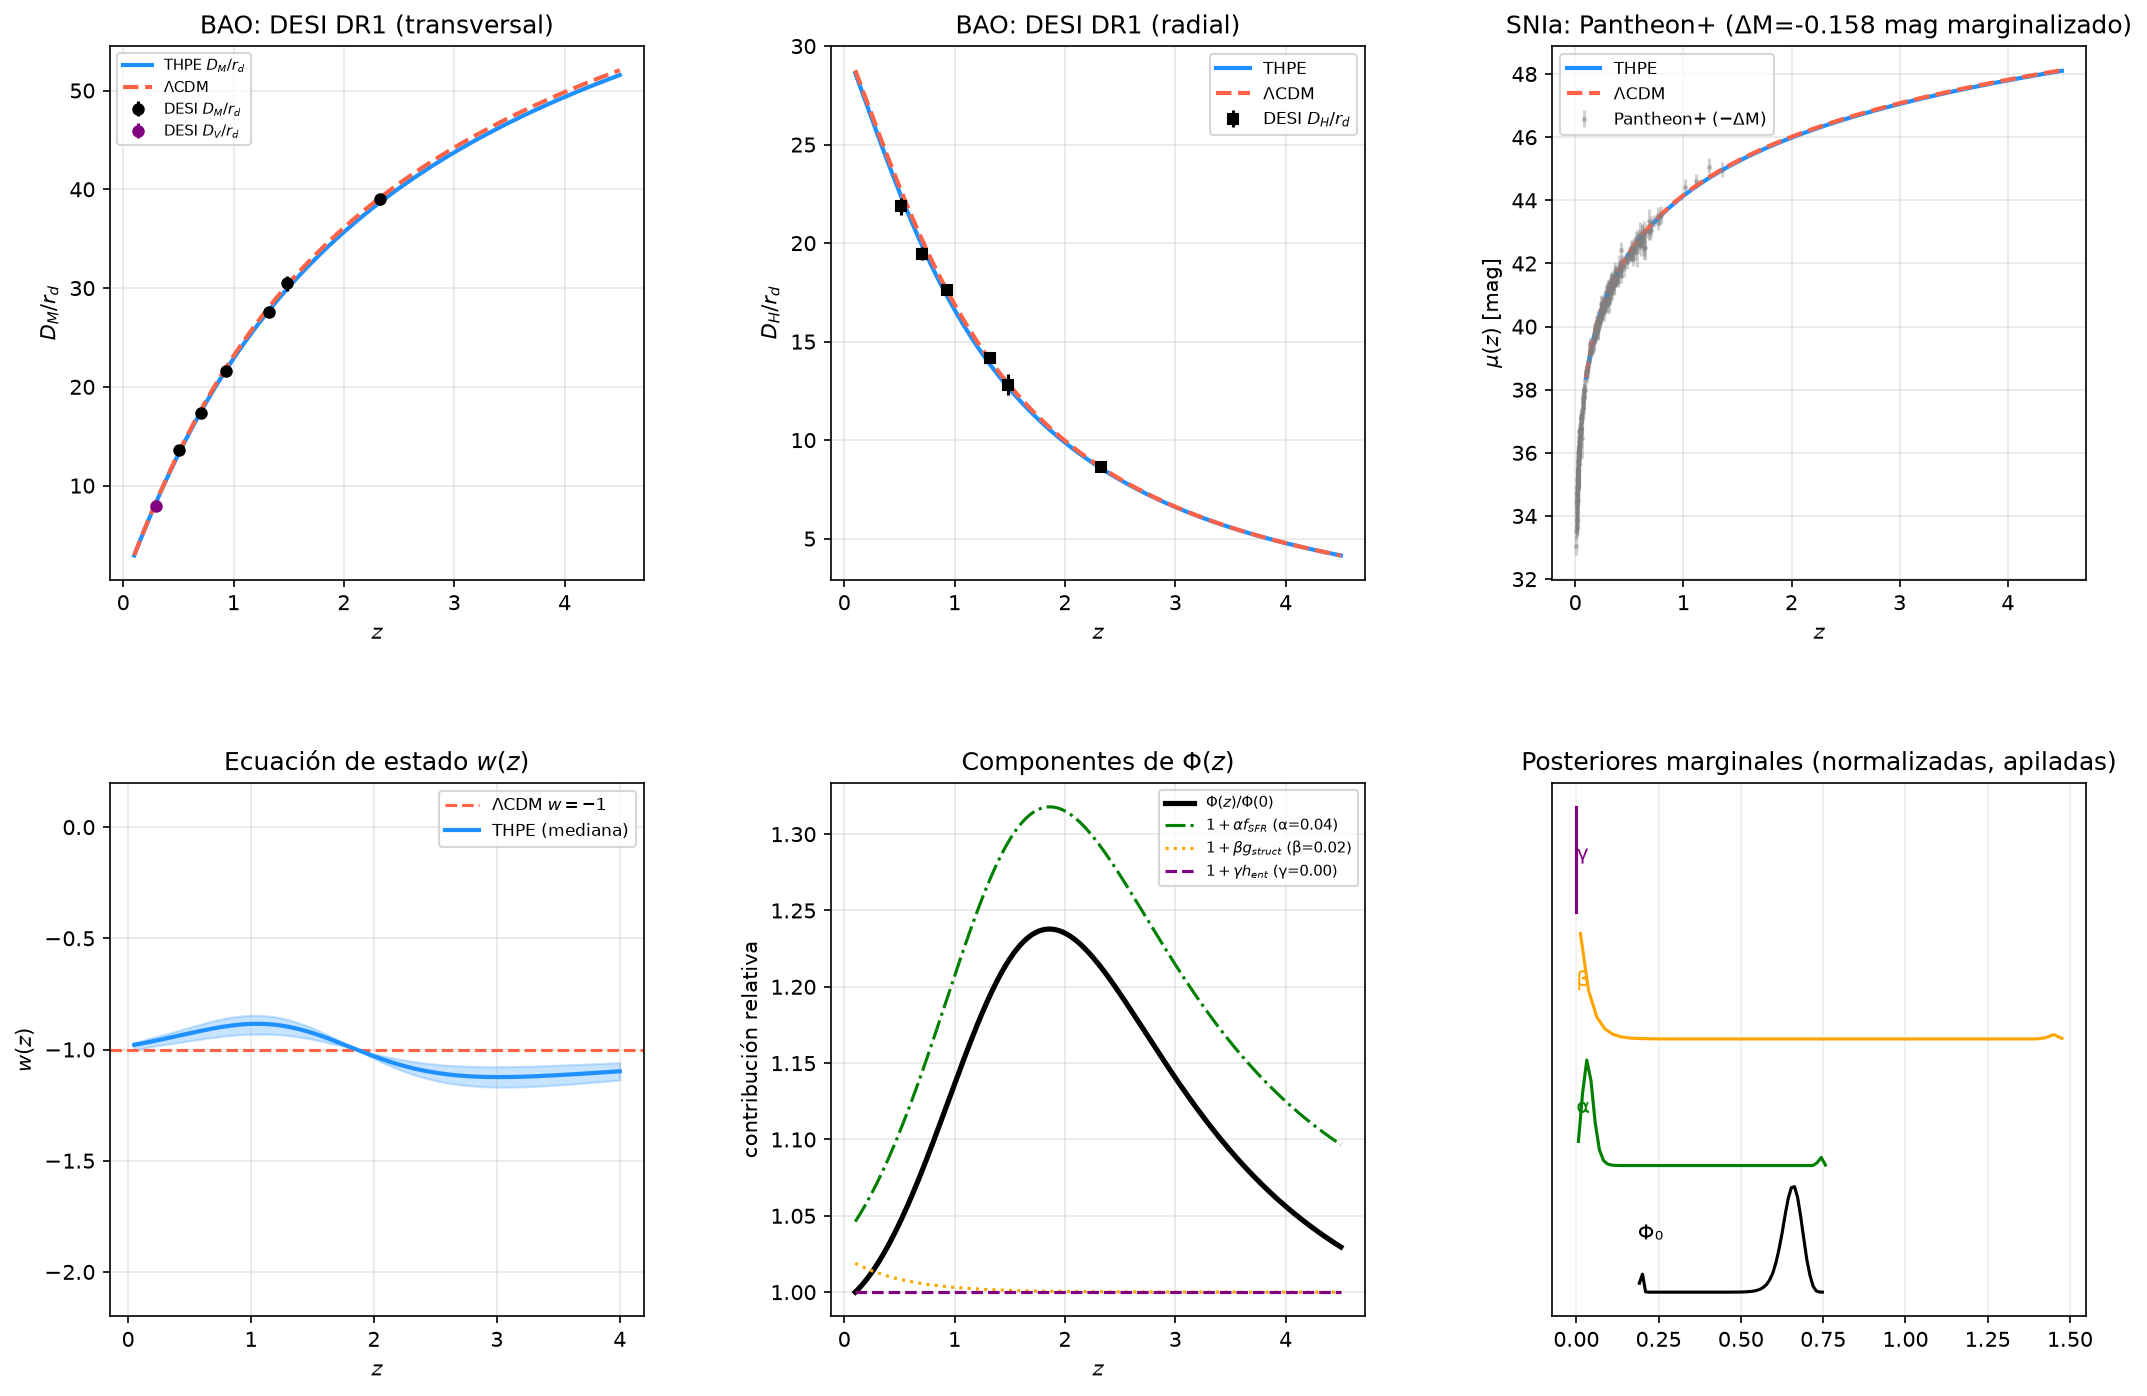
\includegraphics[width=\textwidth]{THPE_v18_dr2_resultados.png}
\caption{Fit of the THPE model to DESI DR2 BAO and Pantheon+ data.
Panels show the transverse and radial BAO observables, the supernova
Hubble diagram with the marginalised magnitude offset applied, the
reconstructed $w(z)$, the individual contributions to $\Phi(z)$, and the
marginal posteriors. The THPE and \LCDM{} curves are indistinguishable
at the resolution of the figure.}
\label{fig:results}
\end{figure*}}{}

\IfFileExists{THPE_v18_dr2_corner.png}{%
\begin{figure}[t]
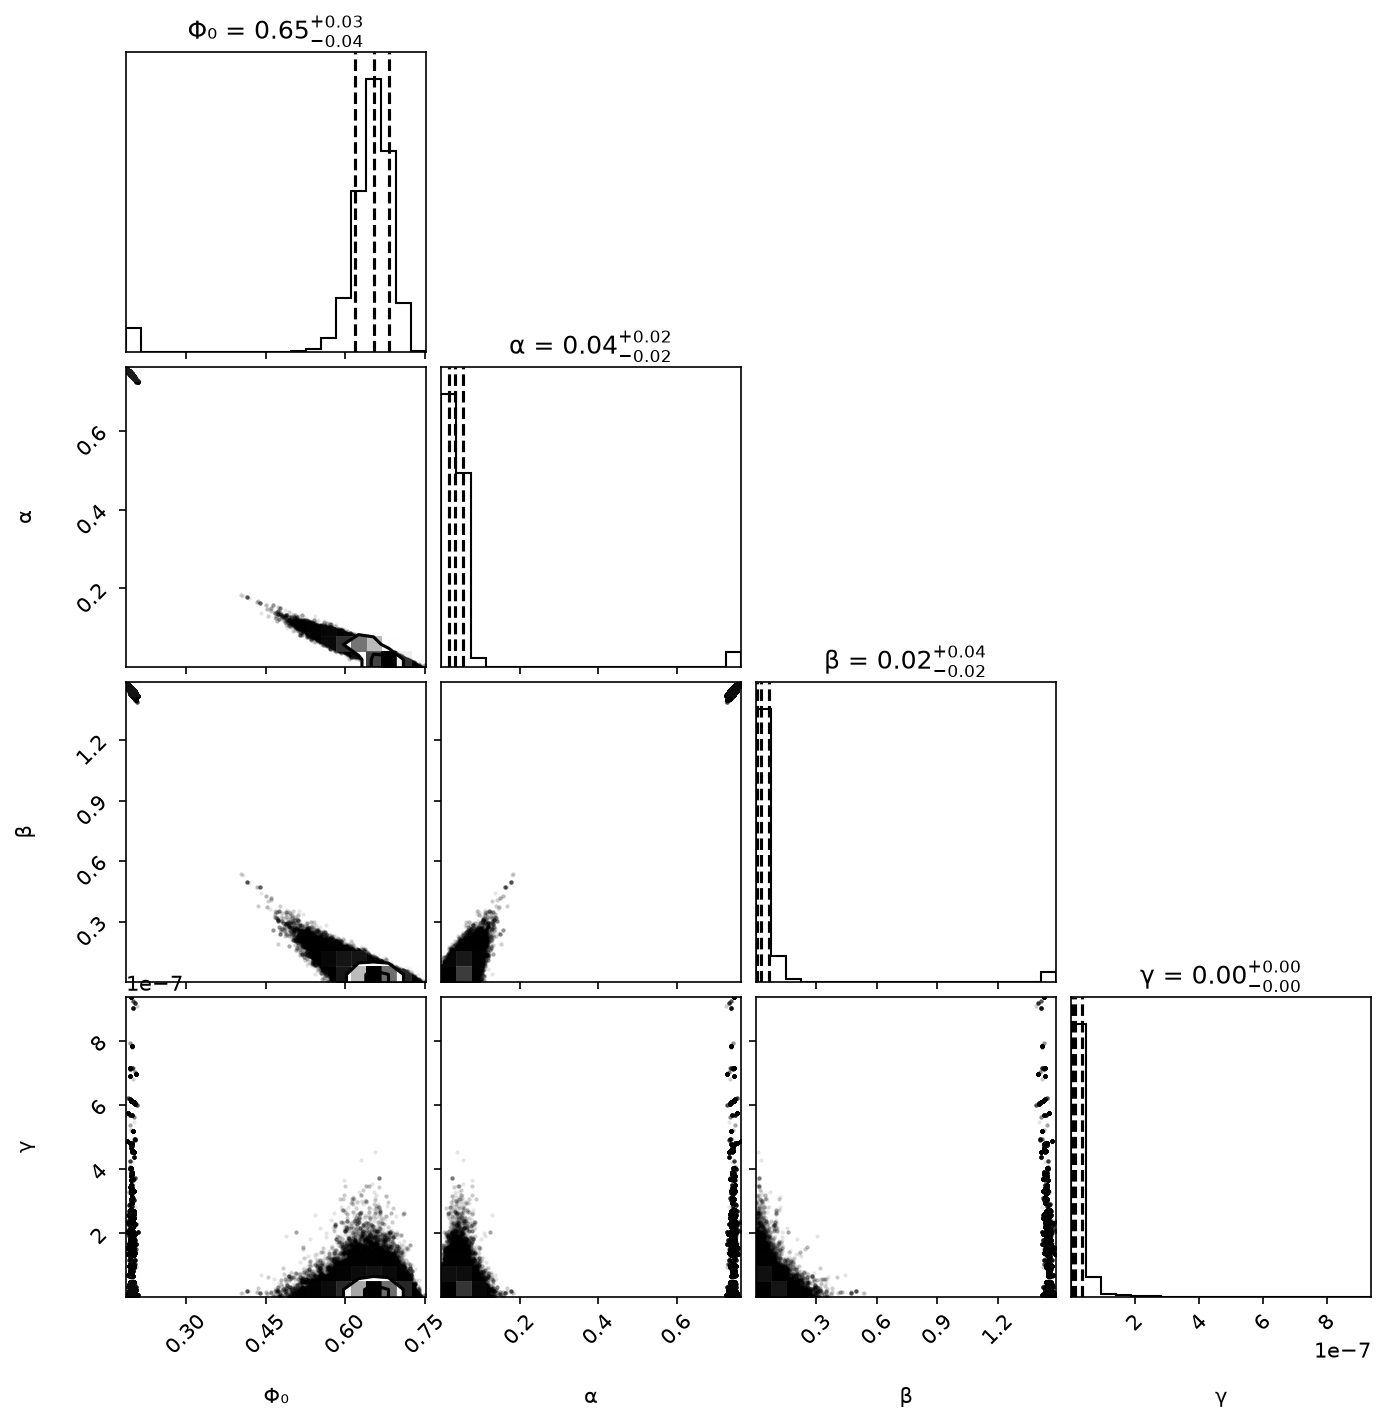
\includegraphics[width=\columnwidth]{THPE_v18_dr2_corner.png}
\caption{Posterior distribution of the four THPE parameters. The
extended $\Phi_0$--$\alpha$--$\beta$ degeneracy is apparent; $\gamma$ is
pinned at zero by the physicality prior.}
\label{fig:corner}
\end{figure}}{}

%=======================================================================
\section{Refutation of the local Compton scale}
\label{sec:compton}
%=======================================================================

An earlier version of the THPE identified the Compton time
$\tau_c=\hbar/Mc^2$ as a universal rate of state compression. Comparing
that scale with experimentally demonstrated quantum coherence times ---
from electron interferometry through molecular interferometry
\cite{Fein2019} to the 40~kg mirrors of LIGO --- the observed coherence
exceeds the prediction by 14 to 51 orders of magnitude across every mass
range ever probed. The identification is therefore refuted.

The only surviving reading of local persistence is strictly relational
(the state $|\psi\rangle$ persists, not a classical trajectory;
compression occurs only through environmental interaction), which is
consistent but operationally equivalent to standard decoherence and thus
carries no additional empirical content. Di\'osi--Penrose-type scales
\cite{Diosi1987,Penrose1996}, $\tau\sim\hbar R/Gm^2$, remain compatible
with all observations and testable with current optomechanics
\cite{Donadi2021}; their exploration lies outside the scope of this
work.

%=======================================================================
\section{Can $\Phi(z)$ be derived?}
\label{sec:derivation}
%=======================================================================

\subsection{Set-up}

We investigated whether Eq.~(\ref{eq:phi}) can be obtained from a
variational principle rather than postulated. The success criterion,
fixed in advance, was to obtain $\Box\Pi=I$ as a \emph{consequence},
with the source $I$ deduced rather than chosen, while passing ghost,
degrees-of-freedom and conservation tests.

\subsection{Minimal case}

Consider the simplest possible non-minimal coupling,
%
\begin{equation}
S=\int d^4x\sqrt{-g}\left[\frac{F(\Pi)R}{2\kappa}
-\frac{\omega}{2}(\partial\Pi)^2-V(\Pi)\right]+S_m,
\label{eq:action}
\end{equation}
%
with $F(\Pi)=1+2\kappa\xi\Pi$. Variation with respect to $\Pi$ gives
%
\begin{equation}
\omega\,\Box\Pi+\xi R-V'(\Pi)=0
\quad\Longrightarrow\quad
\Box\Pi=\frac{V'(\Pi)-\xi R}{\omega}.
\label{eq:boxpi}
\end{equation}
%
The target equation therefore emerges, and the source is \emph{not}
free: $I\propto R$ in vacuum and $I\propto T$ (the trace of the
energy-momment tensor) in the presence of matter, via the trace of the
modified Einstein equations, yielding the canonical Brans--Dicke form
$(2\omega_{\rm BD}+3)\Box\Pi=\kappa T$.

All three consistency tests are passed. In the Einstein frame the
kinetic coefficient is
%
\begin{equation}
K_E=\frac{\omega}{F}+\frac{3}{2\kappa}\left(\frac{F'}{F}\right)^2
=\frac{\omega F+6\kappa\xi^2}{F^2}>0
\quad\text{for }\omega>0,\;F>0,
\label{eq:noghost}
\end{equation}
%
so there is no ghost provided $F>0$ (the region $F<0$ must be excluded
by a physicality prior, in exact analogy with the prior used in the
cosmological analysis). The theory propagates three degrees of freedom
(two tensor, one scalar) with $c_{\rm gw}=c$ exactly, compatible with
GW170817 \cite{GW170817}. Energy--momentum conservation holds
identically because matter couples minimally to $g_{\mu\nu}$ in the
Jordan frame.

\subsection{The bottleneck is local, not cosmological}

The extra scalar mode is precisely that of Brans--Dicke
\cite{BransDicke1961}, with
$\omega_{\rm BD}=\omega F/(F')^2$. The Cassini bound
$\omega_{\rm BD}>4\times10^4$ \cite{Bertotti2003} implies
%
\begin{equation}
|\xi|<2.5\times10^{-3}\kappa^{-1}
\quad\Longrightarrow\quad
\left|\frac{\delta H}{H}\right|<2.5\times10^{-5}.
\label{eq:cassini}
\end{equation}
%
The Solar System limit is thus roughly \emph{400 times more
restrictive} than the cosmological bounds of Eq.~(\ref{eq:bounds}). The
minimal formulation is consistent but indistinguishable from \LCDM{} by
construction --- and would remain so for any future cosmological
dataset.

\subsection{Screening mechanisms}

A field-dependent kinetic term $Z(\Pi)$ cannot produce screening. The
redefinition
%
\begin{equation}
\frac{d\phi}{d\Pi}=\sqrt{Z(\Pi)}
\label{eq:redef}
\end{equation}
%
removes any $Z(\Pi)>0$, returning the theory of
Eq.~(\ref{eq:action}) written in different field-space coordinates; the
effective coupling is $F'/\sqrt{Z}$, a fixed number rather than a
function of the environment. Genuine screening requires dependence on
the local density (chameleon \cite{Khoury2004}, symmetron) or on the
derivatives $X=-(\partial\Pi)^2/2$ (K-mouflage, Vainshtein). The former
are subject to the no-go theorem of Wang, Hui and Khoury
\cite{Wang2012}, which forbids self-acceleration.

\subsection{Vainshtein and Horndeski}
\label{sec:horndeski}

After GW170817, the viable Horndeski Lagrangian reduces to
%
\begin{equation}
\mathcal{L}=G_2(\Pi,X)+G_3(\Pi,X)\Box\Pi+G_4(\Pi)R,
\qquad G_5=0,
\label{eq:horndeski}
\end{equation}
%
and Vainshtein screening \cite{Vainshtein1972} from the $G_3$ term does
resolve Eq.~(\ref{eq:cassini}): the solar Vainshtein radius is
$r_V=(r_s L_c^2)^{1/3}\simeq3.8\times10^{18}$~m $\simeq124$~pc,
suppressing the fifth force by $\sim10^{-9}$ at Neptune's orbit. A
cosmological window between $10^{-3}$ and $10^{-2}$ remains, bounded
above by Eq.~(\ref{eq:bounds}) and further restricted by graviton decay
into dark energy \cite{Creminelli2018} and by gradient-stability
requirements \cite{Kobayashi2019}.

However, the local formulation analysed for $\Pi$ is mathematically
equivalent to a subclass of Galileon/Horndeski theories
\cite{Deffayet2009} within the adopted hypotheses. The retarded
solution of Eq.~(\ref{eq:boxpi}),
%
\begin{equation}
\Pi(x)=\int G_{\rm ret}(x,y)\,I(y)\sqrt{-g}\;d^4y,
\label{eq:retarded}
\end{equation}
%
is a mathematical property of \emph{any} sourced field --- the retarded
Li\'enard--Wiechert potentials have possessed such ``causal memory''
since 1898 --- and adds neither degrees of freedom nor distinctive
predictions.

\subsection{The Planck scale: the real limit of the programme}
\label{sec:planck}

The original intuition placed state persistence at the Planck scale,
$t_P=\sqrt{\hbar G/c^5}\simeq5.4\times10^{-44}$~s, with
$\ell_P=c\,t_P$. Yet the Planck time appears nowhere in the formulation
analysed above: Eq.~(\ref{eq:boxpi}) is a continuous wave equation and
Eq.~(\ref{eq:retarded}) integrates over a continuous past light cone.
Formalising $\Pi$ as a classical field with a covariant action removes
the discreteness by construction.

In this formulation gravity influences $\Pi$ in two ways, neither
involving the Planck scale: as a \emph{source}, through $R$ (and
through $T$ in the presence of matter) in Eq.~(\ref{eq:boxpi}); and as a
\emph{response}, through the $F(\Pi)R$ term, which makes the effective
gravitational constant depend on $\Pi$ and is precisely what
Eq.~(\ref{eq:cassini}) constrains. Both effects are macroscopic and
classical.

This yields a sharper reading of our result: the local formulation does
not fail because of the Cassini bound --- Vainshtein screening resolves
that --- but because, on being made rigorous, it \emph{loses the
ingredient that made it distinctive}. A classical field theory cannot
represent Planck-scale granularity, and without it $\Pi$ is one more
scalar field. If state persistence is genuinely a Planck-scale
phenomenon, its description requires a quantum gravity framework rather
than an effective field theory. We regard this --- rather than the
observational constraints --- as the real limit of the theoretical
programme presented here.

\subsection{Precedent in the literature: Everpresent Lambda}
\label{sec:everpresent}

It is natural to ask whether that route has already been taken. It has.
In causal set theory, Lorentz covariance imposes a Poisson relation
between the spacetime volume of a region and the number $N$ of discrete
elements it contains. From this Sorkin \cite{Sorkin1991,Sorkin2000}
deduced a fluctuating cosmological constant with
$\delta\Lambda\sim1/\sqrt{V}\sim1/\sqrt{N}$: the accumulation of
discrete Planck-scale elements produces, in the macroscopic limit,
dynamical dark energy. The effect is explicitly described as a residual,
non-local quantum consequence of the underlying discreteness
\cite{Ahmed2004,Ahmed2013}. The prediction predates the 1998 discovery
of cosmic acceleration and its order of magnitude agrees with the
observed value without fine-tuning.

The correspondence with the motivation of the present work is close and
we state it explicitly: both start from Planck-scale discrete structure,
both posit that its accumulation affects the expansion, both produce
dynamical dark energy, and both are non-local by construction. The
difference is formal status: Everpresent Lambda \emph{derives} the
fluctuation from a quantum gravity theory, whereas the THPE
\emph{postulated} the functional form of Eq.~(\ref{eq:phi}) from
phenomenological tracers.

That programme is likewise constrained, and by the same observable:
since the everpresent $\Lambda$ originates in past light cones, regions
of the last-scattering surface separated by more than a causal horizon
would carry uncorrelated values, producing CMB anisotropies; the
resulting bound is too small to account for late-time acceleration
\cite{Barrow2007}. The conclusion of Sec.~\ref{sec:horndeski} is
therefore reinforced rather than weakened: the Planck route is not free
territory left unexplored, but ground already covered, formalised and
observationally restricted.

%=======================================================================
\section{Discussion and limitations}
\label{sec:discussion}
%=======================================================================

Three lessons follow. First, the functional form of $\Phi(z)$ is not
what the data require: the DR2--Planck tension projects onto the
amplitude of dark energy rather than its shape. Second, the
$\Phi_0$--$\alpha$--$\beta$ degeneracy is structural; separating the
contributions would require growth observables such as $f\sigma_8$
rather than purely geometric ones. Third, $h_{\rm ent}$ must either be
reformulated from theory, regularising its $z\to0$ divergence, or
dropped.

Limitations are stated explicitly. $H_0$ and $\Omega_m$ are fixed to
Planck values; marginalising over them would broaden the bounds of
Eq.~(\ref{eq:bounds}) without changing the sign of
Eqs.~(\ref{eq:lnB1})--(\ref{eq:lnB2}), which is dominated by the Occam
penalty. We do not use the full CMB likelihood, nor structure growth.
The CMB priors are self-calibrated as described in
Sec.~\ref{sec:data}. The theoretical analysis is restricted to local,
single-field, second-order actions within the space of
Eq.~(\ref{eq:horndeski}); genuinely non-local formulations
\cite{Deser2007}, history functionals, and multi-field sectors are
\emph{not} refuted here --- they were not examined.

%=======================================================================
\section{Conclusions}
\label{sec:conclusions}
%=======================================================================

We have promoted the THPE from proposal to tested hypothesis on two
independent fronts.

Observationally, with the best available public geometric datasets and
explicit validity controls, the evidence strongly favours \LCDM{}
($\ln B$ from $-7.4$ to $-14.8$), excludes the horizon-entropy term, and
bounds informational contributions below $\sim1\%$ of the dark energy
density.

Theoretically, the target equation can be derived from an action
principle, but the resulting local formulation is localised within an
already studied space of theories and provides no independent
phenomenology. The Compton scale is refuted as a physical compression
rate, and the Planck-scale route proves already covered and constrained
in the causal set literature.

The THPE is not falsified: it is \emph{bounded}, and its local
formulation is \emph{closed}. We regard this set of negative results as
a legitimate scientific product: it delimits the viable space of the
hypothesis, documents methodological warnings of general utility (the
non-convergence of ensemble samplers on degenerate posteriors; the
necessity of coherence controls in model comparison), and leaves a
falsifiable prediction with a verifiable time stamp.

%=======================================================================
\section{Future testability}
\label{sec:future}
%=======================================================================

The distinctive prediction of the THPE --- a crossing of $w(z)=-1$ whose
chronology follows the star formation peak at $z\simeq1.9$ --- is
\emph{not} testable at present precision: the permitted couplings,
Eq.~(\ref{eq:bounds}), place the signature below the threshold of
current geometric data.

The datasets that will permit the test are the final DESI release
(expected around 2028--2029, on whatever schedule the collaboration
establishes), the cosmological releases of Euclid \cite{Euclid2011}
(2026--2030), and LSST at the Vera C. Rubin Observatory
\cite{LSST2019} from approximately 2027.

The public, dated registration of this prediction (repository commits of
July 2026) precedes those data. Should dark energy prove dynamical with
the predicted chronology, temporal priority is verifiable; should
$w=-1$ be consolidated at sub-percent precision, the THPE will be
refuted in its reformulations as well, and the authors will say so.

%=======================================================================
\section*{Code and data availability}
%=======================================================================

The complete pipeline, the full correction history and the coherence
controls are publicly available at
\url{https://github.com/moimora1/THPE} (version 1.8):
\texttt{THPE\_fit\_v18.py} (MCMC fit to DESI DR1/DR2 and Pantheon+),
\texttt{THPE\_dynesty\_v1.py} (Bayesian evidence, BAO+SNe) and
\texttt{THPE\_dynesty\_v2\_cmb.py} (evidence with the CMB anchor). The
\texttt{CHANGELOG} documents every version, including the errors
detected and corrected during this work. Pantheon+ data are not
redistributed; the scripts download them from the official
\texttt{PantheonPlusSH0ES/DataRelease} repository.

%=======================================================================
\begin{acknowledgments}
Code development, symbolic and numerical auditing, and technical writing
were assisted by artificial intelligence systems (Claude, Anthropic;
GPT, OpenAI) used with separated roles --- one proposing theoretical
formulations, the other verifying them --- with cross-auditing in both
directions and under human direction throughout. All scientific
decisions and responsibility for the content rest with the human
authors.
\end{acknowledgments}

%%%%%%%%%%%%%%%%%%%%%%%%%%%%%%%%%%%%%%%%%%%%%%%%%%%%%%%%%%%%%%%%%%%%%%%
%  VERSION EN CASTELLANO -- se inserta tras la version inglesa
%%%%%%%%%%%%%%%%%%%%%%%%%%%%%%%%%%%%%%%%%%%%%%%%%%%%%%%%%%%%%%%%%%%%%%%

\clearpage
\onecolumngrid
\begin{center}
\rule{\textwidth}{0.5pt}\\[4pt]
{\large\bfseries VERSI\'ON EN CASTELLANO $\;\vert\;$ SPANISH VERSION}\\[2pt]
{\small Traducci\'on \'integra del art\'iculo precedente. En caso de
discrepancia, prevalece la versi\'on inglesa.}\\[2pt]
{\small\itshape Full translation of the preceding paper. In case of
discrepancy, the English version prevails.}\\[4pt]
\rule{\textwidth}{0.5pt}
\end{center}
\twocolumngrid

\begin{center}
{\large\bfseries La Teor\'ia Hologr\'afica de Persistencia de Estados
confrontada con DESI DR2, Pantheon+ y el CMB: cotas observacionales y
localizaci\'on te\'orica de una extensi\'on informacional de la energ\'ia
oscura hologr\'afica}\\[6pt]
{Mois\'es Mora Garc\'ia y Jorge Ord\'o\~nez Mora}\\[2pt]
{\small Investigadores independientes, Palma de Mallorca, Espa\~na}
\end{center}

\vspace{4pt}

\begin{center}
\begin{minipage}{0.95\columnwidth}
\small
\textbf{Resumen.} Presentamos la Teor\'ia Hologr\'afica de Persistencia
de Estados (THPE), una extensi\'on fenomenol\'ogica de la energ\'ia
oscura hologr\'afica en la que la densidad de energ\'ia oscura se
promueve a un campo
$\Phi(z)=\Phi_0[1+\alpha f_{\rm SFR}(z)+\beta g_{\rm struct}(z)+\gamma
h_{\rm ent}(z)]$ ligado a tres trazadores de complejidad informacional:
la formaci\'on estelar, la estructura a gran escala y la entrop\'ia del
horizonte. El modelo recupera \LCDM{} exactamente para
$\alpha=\beta=\gamma=0$ y predice un cruce de $w(z)=-1$ sincronizado
con la historia de formaci\'on estelar. Reportamos dos resultados
complementarios. (i) Al confrontar el modelo con las oscilaciones
ac\'usticas de bariones de DESI DR2 (13 medidas con correlaciones por
trazador), el compendio de supernovas de tipo Ia Pantheon+ (1588
objetos con la covarianza estad\'istica y sistem\'atica completa y la
calibraci\'on absoluta marginalizada anal\'iticamente) y los priors
comprimidos de distancia del CMB de Planck 2018, el muestreo anidado
arroja $\ln B=-7.4\pm0.2$ a favor de \LCDM{} frente a la variante
m\'inima de un trazador y $\ln B=-14.8\pm0.2$ frente a la de tres
par\'ametros: evidencia fuerte en la escala de Jeffreys en todos los
casos. El t\'ermino de entrop\'ia del horizonte queda excluido por
fisicalidad ($|\gamma|\lesssim10^{-3}$) y las cotas finales son
$\alpha<0.008$ y $\beta<0.07$ (68\% CL), de modo que cualquier
contribuci\'on informacional a la presi\'on hologr\'afica queda por
debajo del $\sim1\%$ de la densidad de energ\'ia oscura.
(ii) Al investigar si $\Phi(z)$ puede derivarse en lugar de postularse,
encontramos que una acci\'on covariante con acoplamiento no m\'inimo
genera efectivamente $\Box\Pi=I$ con la fuente fijada por el
acoplamiento, y que la construcci\'on supera los controles de
fantasmas, grados de libertad y conservaci\'on; sin embargo, la cota de
Cassini sobre el sector escalar resulta $\sim400$ veces m\'as
restrictiva que la cosmolog\'ia, y los mecanismos de apantallamiento
conocidos conducen a teor\'ias ya presentes en la literatura.
Concluimos que la formulaci\'on local escalar--tensorial de la THPE no
proporciona contenido fenomenol\'ogico independiente respecto a las
teor\'ias de Horndeski supervivientes tras GW170817. Mostramos adem\'as
que la identificaci\'on del tiempo de Compton $\tau_c=\hbar/Mc^2$ como
tasa universal de compresi\'on de estados queda refutada por la
coherencia cu\'antica demostrada experimentalmente, por entre 14 y 51
\'ordenes de magnitud. El pipeline completo, sus controles de
coherencia y el historial \'integro de correcciones se hacen p\'ublicos.
La predicci\'on de un cruce de $w=-1$ ligado a la formaci\'on estelar
permanece registrada como test falsable para la pr\'oxima d\'ecada.
\end{minipage}
\end{center}

\vspace{8pt}

%-----------------------------------------------------------------------
\section*{I. Introducci\'on}
%-----------------------------------------------------------------------

La naturaleza de la energ\'ia oscura sigue sin explicaci\'on. Los
resultados recientes de DESI han reabierto la posibilidad de que su
ecuaci\'on de estado evolucione con el tiempo \cite{DESI2024,DESI2025},
lo que motiva el estudio de extensiones din\'amicas de \LCDM{}.

La THPE propone una de ellas: que la densidad de energ\'ia oscura est\'e
ligada al contenido informacional del universo --- la complejidad
generada por la formaci\'on estelar, el crecimiento de estructuras y la
entrop\'ia del horizonte. La motivaci\'on subyacente es que un universo
que produce estructura podr\'ia dejar una huella medible en su propia
expansi\'on.

Este art\'iculo no defiende esa hip\'otesis: la somete a prueba. Una
versi\'on anterior de este trabajo la presentaba como propuesta con
compatibilidad cualitativa. La presente versi\'on reporta el resultado
completo de dos programas de investigaci\'on consecutivos --- uno
observacional y otro matem\'atico ---, ambos con criterios de
aceptaci\'on fijados de antemano y ambos con resultados negativos que
publicamos \'integros. Consideramos que delimitar el espacio viable de
una hip\'otesis es un producto cient\'ifico leg\'itimo.

%-----------------------------------------------------------------------
\section*{II. Marco te\'orico}
%-----------------------------------------------------------------------

\subsection*{A. Formulaci\'on}

La THPE promueve la densidad de energ\'ia oscura a la
Ec.~(\ref{eq:phi}), donde $f_{\rm SFR}$ es la tasa c\'osmica de
formaci\'on estelar normalizada \cite{Madau2014}, $g_{\rm struct}$ una
densidad normalizada de estructura a gran escala y $h_{\rm ent}$ la
entrop\'ia del horizonte por volumen com\'ovil. La ecuaci\'on de
Friedmann resultante es la Ec.~(\ref{eq:friedmann}) y la ecuaci\'on de
estado efectiva la Ec.~(\ref{eq:woz}).

Para $\alpha=\beta=\gamma=0$ se recupera \LCDM{} exactamente, con
$\Phi_0=\Omega_\Lambda$. La predicci\'on caracter\'istica es un cruce de
$w(z)=-1$ cuya cronolog\'ia sigue el m\'aximo de formaci\'on estelar en
$z\simeq1.9$.

\subsection*{B. Relaci\'on con trabajos previos}

La estructura de capas del espacio de Hilbert separadas por el tiempo
de Planck coincide con el marco \emph{Holographic Space-Time} de Banks
y Fischler \cite{Banks2011}; lo declaramos sin reclamar originalidad
sobre ese punto. La contribuci\'on propuesta era el v\'inculo
expl\'icito entre la presi\'on hologr\'afica y trazadores observables de
complejidad. La Secci\'on~VI.H documenta un precedente directo de la
intuici\'on subyacente en la literatura de conjuntos causales.

\subsection*{C. Estatus tras este trabajo}

La Secci\'on~VI muestra que la versi\'on local escalar--tensorial de la
Ec.~(\ref{eq:phi}) se localiza dentro de un espacio de teor\'ias ya
estudiado. En consecuencia, la Ec.~(\ref{eq:phi}) debe entenderse en
este art\'iculo como una \emph{parametrizaci\'on fenomenol\'ogica}
acotada observacionalmente, no como una propuesta de nueva f\'isica
fundamental.

%-----------------------------------------------------------------------
\section*{III. Datos y metodolog\'ia}
%-----------------------------------------------------------------------

\subsection*{A. Datos}

Empleamos tres conjuntos de datos.

\emph{(i) BAO de DESI DR2} \cite{DESI2025}: 13 medidas --- $D_V/r_d$
para el trazador BGS, y los pares $(D_M/r_d,\,D_H/r_d)$ con sus
coeficientes de correlaci\'on para LRG1, LRG2, LRG3+ELG1, ELG2, QSO y
Ly$\alpha$, en el rango $0.295\le z_{\rm eff}\le2.330$. La
transcripci\'on del vector de datos fue verificada contra dos fuentes
independientes.

\emph{(ii) Pantheon+} \cite{Scolnic2022}: 1588 supernovas de tipo Ia
con $z>0.01$ y la matriz de covarianza estad\'istica m\'as
sistem\'atica completa.

\emph{(iii) Priors comprimidos de distancia del CMB} de Planck 2018
\cite{Planck2020,Chen2019}: el par\'ametro de desplazamiento $R$ y la
escala ac\'ustica $\ell_A$ con su correlaci\'on, autocalibrados al
fondo fiducial del pipeline. El desajuste com\'un de modelado
($\sim0.1\%$, procedente del tratamiento de los neutrinos y de la
evaluaci\'on num\'erica de $r_s$) es id\'entico para todos los modelos y
se cancela por construcci\'on; esta elecci\'on se declara
expl\'icitamente.

\subsection*{B. Verosimilitudes}

Para BAO adoptamos una verosimilitud gaussiana con covarianza
bloque-diagonal por trazador. Para las supernovas marginalizamos
anal\'iticamente sobre un desplazamiento constante de magnitud,
Ec.~(\ref{eq:marg}), con $\Delta=\mu_{\rm obs}-\mu_{\rm th}$. Esto hace
el resultado independiente de la calibraci\'on absoluta de SH0ES frente
a Planck. Para el CMB empleamos una gaussiana bidimensional en
$(R,\ell_A)$. El fondo se fija a los valores de Planck 2018
($H_0=67.4~{\rm km\,s^{-1}Mpc^{-1}}$, $\Omega_m=0.315$); esta
limitaci\'on se discute en la Secci\'on~VII.

\subsection*{C. Inferencia}

Priors: $\Phi_0$ log-uniforme en $[10^{-3},2]$; $\alpha$ y $\beta$
uniformes en $[0,10]$; $\gamma$ uniforme en $[0,5]$ (los valores
negativos implican $H^2<0$ en $z\lesssim0.01$, donde existen
supernovas, y se excluyen del prior); se exige $\Phi(z)>0$ en
$0.011\le z\le4.5$. Las evidencias se calculan mediante muestreo
anidado (\textsc{dynesty} \cite{Speagle2020}, $n_{\rm live}=800$,
muestreo por cortes).

Reportamos una advertencia metodol\'ogica de aplicabilidad general: los
muestreadores de conjunto del tipo Goodman--Weare \cite{emcee}
\emph{no} convergen en este posterior. La degeneraci\'on extendida
$\Phi_0$--$\alpha$--$\beta$ produce estad\'isticos de Gelman--Rubin
entre 3 y 8 incluso con 64 cadenas y 20000 pasos. El muestreo anidado
converge y adem\'as proporciona la evidencia.

\subsection*{D. Controles de coherencia}

Se incorporaron dos controles autom\'aticos al pipeline.
\emph{(i) Coherencia del modelo de referencia:} el $\chi^2$ de \LCDM{}
contra cada vector de datos se calcula al arranque y la ejecuci\'on se
aborta si resulta an\'omalo. \emph{(ii) Condici\'on de anidamiento:}
debe cumplirse
$\ln\mathcal{L}_{\rm max}({\rm THPE})\ge
\ln\mathcal{L}_{\rm max}(\Lambda\mathrm{CDM})$, puesto que los modelos
est\'an anidados.

Estos controles detectaron y descartaron tres resultados inv\'alidos
durante la campa\~na. El m\'as instructivo fue un $\ln B=+290$ espurio
\emph{a favor} de la THPE, causado por un truncamiento en la
evaluaci\'on num\'erica del horizonte del sonido ($r_s=139.0$ en lugar
de $144.4$~Mpc). Lo reportamos expl\'icitamente porque ilustra que, en
comparaci\'on bayesiana de modelos, un control de coherencia sobre el
modelo \emph{de referencia} es indispensable: un $\chi^2$ an\'omalo
para el modelo que sabemos que funciona se\~nala un error de
contabilidad, no un descubrimiento.

%-----------------------------------------------------------------------
\section*{IV. Resultados observacionales}
%-----------------------------------------------------------------------

\subsection*{A. Evidencias}

Con el conjunto geom\'etrico completo (BAO de DESI DR2 + Pantheon+ +
priors de distancia del CMB) obtenemos $\ln Z=-740.13\pm0.11$ para
\LCDM{} (1 par\'ametro), $\ln Z=-747.56\pm0.16$ para la THPE con
$\alpha$ \'unicamente (2 par\'ametros) y $\ln Z=-754.92\pm0.19$ para la
THPE con $\gamma=0$ (3 par\'ametros), de donde resultan las
Ecs.~(\ref{eq:lnB1}) y (\ref{eq:lnB2}).

El control de anidamiento se satisface: los tres modelos comparten
$\ln\mathcal{L}_{\rm max}=-733.50$. La configuraci\'on THPE de mejor
ajuste coincide exactamente con \LCDM{} ($\Delta\chi^2=0.0$). Para
\LCDM{} el posterior da $\Phi_0=0.6883$, consistente con el valor de
Planck.

\subsection*{B. Cadena de robustez}

El resultado es estable a lo largo de las combinaciones de datos:
$\Delta{\rm AIC}=+10.5$ con DR1 BAO+SNe mediante MCMC; $\ln B=-11.1$
(3 par\'ametros) y $-4.9$ (solo $\alpha$) con DR2 BAO+SNe mediante
muestreo anidado; y $-14.8$ y $-7.4$ respectivamente al a\~nadir el
ancla del CMB.

A\~nadir el ancla del CMB \emph{empeora} el caso de la THPE. Sin ella,
\LCDM{} prefiere $\Phi_0=0.724>0.685$, rompiendo la planitud: la
tensi\'on suave ($\sim2.3\sigma$) entre DR2 y Planck se proyecta sobre
la \emph{amplitud} de la energ\'ia oscura, no sobre su forma funcional,
y ni $f_{\rm SFR}$ ni $g_{\rm struct}$ poseen la forma requerida.

\subsection*{C. Cotas de par\'ametros}

Al 68\% de credibilidad se obtienen las cotas de la
Ec.~(\ref{eq:bounds}). El t\'ermino de entrop\'ia del horizonte queda
excluido tal como fue formulado: con la normalizaci\'on adoptada,
$h_{\rm ent}$ diverge como $z^{-3}$ cuando $z\to0$, de modo que la
positividad de $H^2$ donde existen supernovas, junto con las distancias
de las supernovas cercanas, confina $\gamma$ a cero. Cualquier
contribuci\'on informacional a la presi\'on hologr\'afica queda por
tanto por debajo del $\sim1\%$ de la densidad de energ\'ia oscura.

La direcci\'on de degeneraci\'on est\'a bien determinada,
$\Phi_0(1+\alpha+\beta)\simeq\Omega_\Lambda$: el ajuste distribuye la
misma amplitud de energ\'ia oscura entre tres par\'ametros.

%-----------------------------------------------------------------------
\section*{V. Refutaci\'on de la escala local de Compton}
%-----------------------------------------------------------------------

Una versi\'on anterior de la THPE identificaba el tiempo de Compton
$\tau_c=\hbar/Mc^2$ como tasa universal de compresi\'on de estados. Al
comparar esa escala con los tiempos de coherencia cu\'antica
demostrados experimentalmente --- desde la interferometr\'ia de
electrones, pasando por la interferometr\'ia molecular \cite{Fein2019},
hasta los espejos de 40~kg de LIGO ---, la coherencia observada excede
la predicci\'on por entre 14 y 51 \'ordenes de magnitud en todos los
rangos de masa jam\'as sondeados. La identificaci\'on queda por tanto
refutada.

La \'unica lectura superviviente de la persistencia local es
estrictamente relacional (persiste el estado $|\psi\rangle$, no una
trayectoria cl\'asica; la compresi\'on ocurre \'unicamente por
interacci\'on con el entorno), que es consistente pero operacionalmente
equivalente a la decoherencia est\'andar y por tanto carece de
contenido emp\'irico adicional. Las escalas de tipo Di\'osi--Penrose
\cite{Diosi1987,Penrose1996}, $\tau\sim\hbar R/Gm^2$, permanecen
compatibles con todas las observaciones y son contrastables con la
optomec\'anica actual \cite{Donadi2021}; su exploraci\'on queda fuera
del alcance de este trabajo.

%-----------------------------------------------------------------------
\section*{VI. ¿Puede derivarse $\Phi(z)$?}
%-----------------------------------------------------------------------

\subsection*{A. Planteamiento}

Investigamos si la Ec.~(\ref{eq:phi}) puede obtenerse de un principio
variacional en lugar de postularse. El criterio de \'exito, fijado de
antemano, era obtener $\Box\Pi=I$ como \emph{consecuencia}, con la
fuente $I$ deducida y no elegida, superando los controles de
fantasmas, grados de libertad y conservaci\'on.

\subsection*{B. Caso m\'inimo}

Consideramos el acoplamiento no m\'inimo m\'as simple posible,
Ec.~(\ref{eq:action}), con $F(\Pi)=1+2\kappa\xi\Pi$. La variaci\'on
respecto a $\Pi$ conduce a la Ec.~(\ref{eq:boxpi}).

La ecuaci\'on objetivo emerge, por tanto, y la fuente \emph{no} es
libre: $I\propto R$ en vac\'io e $I\propto T$ (la traza del tensor
energ\'ia--momento) en presencia de materia, a trav\'es de la traza de
las ecuaciones de Einstein modificadas, dando la forma can\'onica de
Brans--Dicke $(2\omega_{\rm BD}+3)\Box\Pi=\kappa T$.

Se superan los tres controles de consistencia. En el marco de Einstein
el coeficiente cin\'etico viene dado por la Ec.~(\ref{eq:noghost}), de
modo que no hay fantasma siempre que $F>0$ (la regi\'on $F<0$ debe
excluirse mediante un prior de fisicalidad, en analog\'ia exacta con el
prior empleado en el an\'alisis cosmol\'ogico). La teor\'ia propaga tres
grados de libertad (dos tensoriales y uno escalar) con
$c_{\rm gw}=c$ exactamente, compatible con GW170817 \cite{GW170817}. La
conservaci\'on del tensor energ\'ia--momento se cumple id\'enticamente
porque la materia se acopla m\'inimamente a $g_{\mu\nu}$ en el marco de
Jordan.

\subsection*{C. El cuello de botella es local, no cosmol\'ogico}

El modo escalar adicional es precisamente el de Brans--Dicke
\cite{BransDicke1961}, con $\omega_{\rm BD}=\omega F/(F')^2$. La cota
de Cassini $\omega_{\rm BD}>4\times10^4$ \cite{Bertotti2003} implica la
Ec.~(\ref{eq:cassini}). El l\'imite del Sistema Solar resulta as\'i
aproximadamente \emph{400 veces m\'as restrictivo} que las cotas
cosmol\'ogicas de la Ec.~(\ref{eq:bounds}). La formulaci\'on m\'inima es
consistente pero indistinguible de \LCDM{} por construcci\'on --- y lo
seguir\'ia siendo ante cualquier conjunto de datos cosmol\'ogicos
futuro.

\subsection*{D. Mecanismos de apantallamiento}

Un t\'ermino cin\'etico $Z(\Pi)$ dependiente del campo no puede
producir apantallamiento. La redefinici\'on de la
Ec.~(\ref{eq:redef}) elimina cualquier $Z(\Pi)>0$ y devuelve la teor\'ia
de la Ec.~(\ref{eq:action}) escrita en otras coordenadas del espacio de
campos; el acoplamiento efectivo resultante es $F'/\sqrt{Z}$, un
n\'umero fijo y no una funci\'on del entorno. Un apantallamiento
genuino requiere dependencia de la densidad local (camale\'on
\cite{Khoury2004}, simetr\'on) o de las derivadas
$X=-(\partial\Pi)^2/2$ (K-mouflage, Vainshtein). Los primeros est\'an
sujetos al teorema no-go de Wang, Hui y Khoury \cite{Wang2012}, que
proh\'ibe la autoaceleraci\'on.

\subsection*{E. Vainshtein y Horndeski}

Tras GW170817, el lagrangiano de Horndeski viable se reduce a la
Ec.~(\ref{eq:horndeski}), y el apantallamiento de Vainshtein
\cite{Vainshtein1972} procedente del t\'ermino $G_3$ s\'i resuelve la
Ec.~(\ref{eq:cassini}): el radio de Vainshtein solar es
$r_V=(r_s L_c^2)^{1/3}\simeq3.8\times10^{18}$~m $\simeq124$~pc, con una
supresi\'on de la quinta fuerza de $\sim10^{-9}$ en la \'orbita de
Neptuno. Queda una ventana cosmol\'ogica entre $10^{-3}$ y $10^{-2}$,
acotada superiormente por la Ec.~(\ref{eq:bounds}) y restringida
adem\'as por el decaimiento de gravitones en energ\'ia oscura
\cite{Creminelli2018} y por los requisitos de estabilidad de gradiente
\cite{Kobayashi2019}.

Sin embargo, la formulaci\'on local analizada para $\Pi$ resulta
matem\'aticamente equivalente a una subclase de teor\'ias
galile\'on/Horndeski \cite{Deffayet2009} dentro de las hip\'otesis
adoptadas. La soluci\'on retardada de la Ec.~(\ref{eq:boxpi}), dada por
la Ec.~(\ref{eq:retarded}), es una propiedad matem\'atica de
\emph{cualquier} campo con fuente --- los potenciales retardados de
Li\'enard--Wiechert poseen esa ``memoria causal'' desde 1898 --- y no
a\~nade grados de libertad ni predicciones distintivas.

\subsection*{F. La escala de Planck: el l\'imite real del programa}

La intuici\'on original situaba la persistencia de estados en la escala
de Planck, $t_P=\sqrt{\hbar G/c^5}\simeq5.4\times10^{-44}$~s, con
$\ell_P=c\,t_P$. Sin embargo, el tiempo de Planck no aparece en ning\'un
punto de la formulaci\'on analizada: la Ec.~(\ref{eq:boxpi}) es una
ecuaci\'on de ondas continua y la Ec.~(\ref{eq:retarded}) integra sobre
un cono de luz pasado continuo. Formalizar $\Pi$ como campo cl\'asico
con una acci\'on covariante elimina la discretizaci\'on por
construcci\'on.

En esta formulaci\'on la gravedad influye sobre $\Pi$ de dos maneras,
ninguna de las cuales involucra la escala de Planck: como
\emph{fuente}, a trav\'es de $R$ (y de $T$ en presencia de materia) en
la Ec.~(\ref{eq:boxpi}); y como \emph{respuesta}, a trav\'es del
t\'ermino $F(\Pi)R$, que hace que la constante gravitatoria efectiva
dependa de $\Pi$ y es precisamente lo que restringe la
Ec.~(\ref{eq:cassini}). Ambos efectos son macrosc\'opicos y cl\'asicos.

De aqu\'i se sigue una lectura m\'as precisa de nuestro resultado: la
formulaci\'on local no fracasa por la cota de Cassini --- el
apantallamiento de Vainshtein la resuelve --- sino porque, al hacerse
rigurosa, \emph{pierde el ingrediente que la hac\'ia distintiva}. Una
teor\'ia cl\'asica de campos no puede representar granularidad a escala
de Planck, y sin ella $\Pi$ es un campo escalar m\'as. Si la
persistencia de estados es genuinamente un fen\'omeno de escala de
Planck, su descripci\'on exige un marco de gravedad cu\'antica y no una
teor\'ia efectiva de campos. Consideramos que este --- y no las
restricciones observacionales --- es el l\'imite real del programa
te\'orico presentado aqu\'i.

\subsection*{G. Precedente en la literatura: \emph{Everpresent Lambda}}

Cabe preguntarse si esa v\'ia ha sido ya recorrida. Lo ha sido. En la
teor\'ia de conjuntos causales, la covariancia Lorentz impone una
relaci\'on de Poisson entre el volumen espacio-temporal de una regi\'on
y el n\'umero $N$ de elementos discretos que contiene. De ah\'i Sorkin
\cite{Sorkin1991,Sorkin2000} dedujo una constante cosmol\'ogica
fluctuante con $\delta\Lambda\sim1/\sqrt{V}\sim1/\sqrt{N}$: la
acumulaci\'on de elementos discretos a escala de Planck produce, en el
l\'imite macrosc\'opico, energ\'ia oscura din\'amica. El efecto se
describe expl\'icitamente como una consecuencia cu\'antica residual y no
local de la discretizaci\'on subyacente \cite{Ahmed2004,Ahmed2013}. La
predicci\'on es anterior al descubrimiento de la aceleraci\'on
c\'osmica de 1998 y su orden de magnitud concuerda con el valor
observado sin ajuste fino.

La correspondencia con la motivaci\'on del presente trabajo es estrecha
y la declaramos expl\'icitamente: ambos parten de una estructura
discreta a escala de Planck, ambos postulan que su acumulaci\'on afecta
a la expansi\'on, ambos producen energ\'ia oscura din\'amica y ambos son
no locales por construcci\'on. La diferencia es de estatus formal:
\emph{Everpresent Lambda} \emph{deriva} la fluctuaci\'on desde una
teor\'ia de gravedad cu\'antica, mientras que la THPE \emph{postulaba}
la forma funcional de la Ec.~(\ref{eq:phi}) a partir de trazadores
fenomenol\'ogicos.

Ese programa est\'a asimismo restringido, y por el mismo observable:
puesto que el $\Lambda$ omnipresente se origina en los conos de luz
pasados, regiones de la superficie de \'ultima dispersi\'on separadas
por m\'as de un horizonte causal portar\'ian valores no correlacionados,
produciendo anisotrop\'ias en el CMB; la cota resultante es demasiado
peque\~na para dar cuenta de la aceleraci\'on tard\'ia
\cite{Barrow2007}. La conclusi\'on de la Secci\'on~VI.E queda por tanto
reforzada, y no debilitada: la v\'ia de Planck no es territorio libre
pendiente de explorar, sino terreno ya recorrido, formalizado y
observacionalmente restringido.

%-----------------------------------------------------------------------
\section*{VII. Discusi\'on y limitaciones}
%-----------------------------------------------------------------------

Se siguen tres lecciones. Primera, la forma funcional de $\Phi(z)$ no es
la que los datos requieren: la tensi\'on DR2--Planck se proyecta sobre
la amplitud de la energ\'ia oscura antes que sobre su forma. Segunda, la
degeneraci\'on $\Phi_0$--$\alpha$--$\beta$ es estructural; separar las
contribuciones requerir\'ia observables de crecimiento como $f\sigma_8$
en lugar de observables puramente geom\'etricos. Tercera,
$h_{\rm ent}$ debe reformularse desde la teor\'ia, regularizando su
divergencia en $z\to0$, o bien eliminarse.

Las limitaciones se declaran expl\'icitamente. $H_0$ y $\Omega_m$ se
fijan a los valores de Planck; marginalizar sobre ellos ensanchar\'ia
las cotas de la Ec.~(\ref{eq:bounds}) sin alterar el signo de las
Ecs.~(\ref{eq:lnB1})--(\ref{eq:lnB2}), dominado por la penalizaci\'on de
Occam. No empleamos la verosimilitud completa del CMB ni el crecimiento
de estructuras. Los priors del CMB est\'an autocalibrados seg\'un se
describe en la Secci\'on~III.A. El an\'alisis te\'orico se restringe a
acciones locales, de un solo campo y de segundo orden dentro del
espacio de la Ec.~(\ref{eq:horndeski}); las formulaciones genuinamente
no locales \cite{Deser2007}, los funcionales de historia y los sectores
multicampo \emph{no} quedan refutados aqu\'i: no fueron examinados.

%-----------------------------------------------------------------------
\section*{VIII. Conclusiones}
%-----------------------------------------------------------------------

Hemos promovido la THPE de propuesta a hip\'otesis contrastada en dos
frentes independientes.

Observacionalmente, con los mejores conjuntos p\'ublicos de datos
geom\'etricos disponibles y con controles de validez expl\'icitos, la
evidencia favorece fuertemente a \LCDM{} ($\ln B$ entre $-7.4$ y
$-14.8$), excluye el t\'ermino de entrop\'ia del horizonte y acota las
contribuciones informacionales por debajo del $\sim1\%$ de la densidad
de energ\'ia oscura.

Te\'oricamente, la ecuaci\'on objetivo puede derivarse de un principio
variacional, pero la formulaci\'on local resultante se localiza dentro
de un espacio de teor\'ias ya estudiado y no proporciona fenomenolog\'ia
independiente. La escala de Compton queda refutada como tasa f\'isica de
compresi\'on, y la v\'ia de escala de Planck resulta ya recorrida y
restringida en la literatura de conjuntos causales.

La THPE no queda falsada: queda \emph{acotada}, y su formulaci\'on local
queda \emph{cerrada}. Consideramos este conjunto de resultados
negativos un producto cient\'ifico leg\'itimo: delimita el espacio
viable de la hip\'otesis, documenta advertencias metodol\'ogicas de
utilidad general (la no convergencia de los muestreadores de conjunto
en posteriors degenerados; la necesidad de controles de coherencia en
la comparaci\'on de modelos) y deja una predicci\'on falsable con
marca temporal verificable.

%-----------------------------------------------------------------------
\section*{IX. Contrastabilidad futura}
%-----------------------------------------------------------------------

La predicci\'on distintiva de la THPE --- un cruce de $w(z)=-1$ cuya
cronolog\'ia sigue el m\'aximo de formaci\'on estelar en $z\simeq1.9$
--- \emph{no} es contrastable con la precisi\'on actual: los
acoplamientos permitidos, Ec.~(\ref{eq:bounds}), sit\'uan la firma por
debajo del umbral de los datos geom\'etricos disponibles.

Los conjuntos de datos que permitir\'an el test son la liberaci\'on
final de DESI (esperada hacia 2028--2029, en el calendario que la
colaboraci\'on establezca), las liberaciones cosmol\'ogicas de Euclid
\cite{Euclid2011} (2026--2030) y LSST en el Observatorio Vera C. Rubin
\cite{LSST2019} desde aproximadamente 2027.

El registro p\'ublico y fechado de esta predicci\'on (\emph{commits} del
repositorio de julio de 2026) precede a esos datos. Si la energ\'ia
oscura resultase din\'amica con la cronolog\'ia predicha, la prioridad
temporal es verificable; si $w=-1$ se consolidase con precisi\'on
inferior al uno por ciento, la THPE quedar\'a refutada tambi\'en en sus
reformulaciones, y los autores as\'i lo har\'an constar.

%-----------------------------------------------------------------------
\section*{Disponibilidad de c\'odigo y datos}
%-----------------------------------------------------------------------

El pipeline completo, el historial \'integro de correcciones y los
controles de coherencia est\'an disponibles p\'ublicamente en
\url{https://github.com/moimora1/THPE} (versi\'on 1.8):
\texttt{THPE\_fit\_v18.py} (ajuste MCMC a DESI DR1/DR2 y Pantheon+),
\texttt{THPE\_dynesty\_v1.py} (evidencia bayesiana, BAO+SNe) y
\texttt{THPE\_dynesty\_v2\_cmb.py} (evidencia con el ancla del CMB). El
\texttt{CHANGELOG} documenta cada versi\'on, incluidos los errores
detectados y corregidos durante este trabajo. Los datos de Pantheon+ no
se redistribuyen; los scripts los descargan del repositorio oficial
\texttt{PantheonPlusSH0ES/DataRelease}.

%-----------------------------------------------------------------------
\section*{Agradecimientos}
%-----------------------------------------------------------------------

El desarrollo del c\'odigo, la auditor\'ia simb\'olica y num\'erica y la
redacci\'on t\'ecnica contaron con la asistencia de sistemas de
inteligencia artificial (Claude, Anthropic; GPT, OpenAI) empleados con
roles separados --- uno proponiendo formulaciones te\'oricas y otro
verific\'andolas ---, con auditor\'ia cruzada en ambas direcciones y
bajo direcci\'on humana en todo momento. Todas las decisiones
cient\'ificas y la responsabilidad sobre el contenido corresponden a los
autores humanos.


%=======================================================================
\begin{thebibliography}{99}

\bibitem{DESI2024} DESI Collaboration, \emph{DESI 2024 VI:
Cosmological Constraints from the Measurements of Baryon Acoustic
Oscillations}, arXiv:2404.03002.

\bibitem{DESI2025} DESI Collaboration, \emph{DESI DR2 Results II:
Measurements of Baryon Acoustic Oscillations and Cosmological
Constraints}, arXiv:2503.14738.

\bibitem{Madau2014} P.~Madau and M.~Dickinson,
Annu. Rev. Astron. Astrophys. \textbf{52}, 415 (2014).

\bibitem{Banks2011} T.~Banks and W.~Fischler,
\emph{Holographic Space-Time}, arXiv:1109.2435.

\bibitem{Scolnic2022} D.~Scolnic \emph{et al.},
Astrophys. J. \textbf{938}, 113 (2022).

\bibitem{Planck2020} Planck Collaboration,
Astron. Astrophys. \textbf{641}, A6 (2020).

\bibitem{Chen2019} L.~Chen, Q.-G.~Huang and K.~Wang,
J. Cosmol. Astropart. Phys. \textbf{02}, 028 (2019).

\bibitem{Speagle2020} J.~S.~Speagle,
Mon. Not. R. Astron. Soc. \textbf{493}, 3132 (2020).

\bibitem{emcee} D.~Foreman-Mackey, D.~W.~Hogg, D.~Lang and J.~Goodman,
Publ. Astron. Soc. Pac. \textbf{125}, 306 (2013).

\bibitem{Fein2019} Y.~Y.~Fein \emph{et al.},
Nat. Phys. \textbf{15}, 1242 (2019).

\bibitem{Diosi1987} L.~Di\'osi, Phys. Lett. A \textbf{120}, 377 (1987).

\bibitem{Penrose1996} R.~Penrose,
Gen. Relativ. Gravit. \textbf{28}, 581 (1996).

\bibitem{Donadi2021} S.~Donadi \emph{et al.},
Nat. Phys. \textbf{17}, 74 (2021).

\bibitem{GW170817} B.~P.~Abbott \emph{et al.} (LIGO Scientific
Collaboration, Virgo Collaboration, Fermi-GBM and INTEGRAL),
Astrophys. J. Lett. \textbf{848}, L13 (2017).

\bibitem{BransDicke1961} C.~Brans and R.~H.~Dicke,
Phys. Rev. \textbf{124}, 925 (1961).

\bibitem{Bertotti2003} B.~Bertotti, L.~Iess and P.~Tortora,
Nature \textbf{425}, 374 (2003).

\bibitem{Khoury2004} J.~Khoury and A.~Weltman,
Phys. Rev. Lett. \textbf{93}, 171104 (2004).

\bibitem{Wang2012} J.~Wang, L.~Hui and J.~Khoury,
Phys. Rev. Lett. \textbf{109}, 241301 (2012).

\bibitem{Vainshtein1972} A.~I.~Vainshtein,
Phys. Lett. B \textbf{39}, 393 (1972).

\bibitem{Deffayet2009} C.~Deffayet, G.~Esposito-Far\`ese and A.~Vikman,
Phys. Rev. D \textbf{79}, 084003 (2009).

\bibitem{Creminelli2018} P.~Creminelli, M.~Lewandowski, G.~Tambalo and
F.~Vernizzi, J. Cosmol. Astropart. Phys. \textbf{12}, 025 (2018).

\bibitem{Kobayashi2019} T.~Kobayashi,
Rep. Prog. Phys. \textbf{82}, 086901 (2019).

\bibitem{Deser2007} S.~Deser and R.~P.~Woodard,
Phys. Rev. Lett. \textbf{99}, 111301 (2007).

\bibitem{Sorkin1991} R.~D.~Sorkin, in \emph{Relativity and Gravitation:
Classical and Quantum} (Proc. SILARG VII, Cocoyoc, Mexico, 1990),
World Scientific, p.~150.

\bibitem{Sorkin2000} R.~D.~Sorkin,
Int. J. Theor. Phys. \textbf{39}, 1731 (2000).

\bibitem{Ahmed2004} M.~Ahmed, S.~Dodelson, P.~B.~Greene and
R.~D.~Sorkin, Phys. Rev. D \textbf{69}, 103523 (2004).

\bibitem{Ahmed2013} M.~Ahmed and R.~D.~Sorkin,
Phys. Rev. D \textbf{87}, 063515 (2013).

\bibitem{Barrow2007} J.~D.~Barrow,
Phys. Rev. D \textbf{75}, 067301 (2007);
see also M.~Ahmed \emph{et al.}, arXiv:0711.2904.

\bibitem{Euclid2011} R.~Laureijs \emph{et al.},
\emph{Euclid Definition Study Report}, arXiv:1110.3193.

\bibitem{LSST2019} \v{Z}.~Ivezi\'c \emph{et al.},
Astrophys. J. \textbf{873}, 111 (2019).

\end{thebibliography}

\end{document}

%%%%%%%%%%%%%%%%%%%%%%%%%%%%%%%%%%%%%%%%%%%%%%%%%%%%%%%%%%%%%%%%%%%%%%%
%  The Holographic Theory of State Persistence confronted with
%  DESI DR2, Pantheon+ and the CMB
%
%  Moises Mora Garcia & Jorge Ordonez Mora
%  Palma de Mallorca, Spain -- 2026
%
%  Compile with:  pdflatex THPE_arxiv_EN.tex   (twice, for references)
%  Requires: revtex4-2 (standard in TeX Live / MiKTeX)
%
%  NOTE FOR THE AUTHORS: figures THPE_v18_dr2_resultados.png and
%  THPE_v18_dr2_corner.png must be in the same folder as this file.
%  If they are absent the document still compiles (figures are wrapped
%  in \IfFileExists), but the figure slots will be empty.
%%%%%%%%%%%%%%%%%%%%%%%%%%%%%%%%%%%%%%%%%%%%%%%%%%%%%%%%%%%%%%%%%%%%%%%

\documentclass[aps,prd,twocolumn,superscriptaddress,nofootinbib,floatfix]{revtex4-2}

\usepackage{amsmath,amssymb}
\usepackage{graphicx}
\usepackage{hyperref}
\hypersetup{colorlinks=true,linkcolor=blue,citecolor=blue,urlcolor=blue}
\usepackage[utf8]{inputenc}

\newcommand{\LCDM}{\ensuremath{\Lambda}CDM}
\newcommand{\Msun}{M_\odot}

\begin{document}

\title{The Holographic Theory of State Persistence confronted with
DESI DR2, Pantheon+ and the CMB: observational bounds and theoretical
localisation of an informational extension of holographic dark energy}

\author{Mois\'es Mora Garc\'ia}
\affiliation{Independent researcher, Palma de Mallorca, Spain}
\author{Jorge Ord\'o\~nez Mora}
\affiliation{Independent researcher, Palma de Mallorca, Spain}

\date{\today}

\begin{abstract}
We present the Holographic Theory of State Persistence (THPE), a
phenomenological extension of holographic dark energy in which the dark
energy density is promoted to a field
$\Phi(z)=\Phi_0[1+\alpha f_{\rm SFR}(z)+\beta g_{\rm struct}(z)+\gamma
h_{\rm ent}(z)]$ tied to three tracers of informational complexity:
star formation, large-scale structure and horizon entropy. The model
recovers \LCDM{} exactly for $\alpha=\beta=\gamma=0$ and predicts a
crossing of $w(z)=-1$ synchronised with the star formation history.
We report two complementary results. (i) Confronting the model with
DESI DR2 baryon acoustic oscillations (13 measurements with per-tracer
correlations), the Pantheon+ Type~Ia supernova compilation (1588
objects with the full statistical-plus-systematic covariance and the
absolute calibration analytically marginalised) and the compressed CMB
distance priors from Planck 2018, nested sampling yields
$\ln B=-7.4\pm0.2$ in favour of \LCDM{} against the minimal
single-tracer variant and $\ln B=-14.8\pm0.2$ against the
three-parameter variant: strong evidence on the Jeffreys scale in all
cases. The horizon-entropy term is excluded by physicality
($|\gamma|\lesssim10^{-3}$) and the final bounds are $\alpha<0.008$ and
$\beta<0.07$ (68\% CL), so that any informational contribution to the
holographic pressure lies below $\sim1\%$ of the dark energy density.
(ii) Investigating whether $\Phi(z)$ can be derived rather than
postulated, we find that a covariant action with non-minimal coupling
does generate $\Box\Pi=I$ with the source fixed by the coupling, and
that the construction passes ghost, degrees-of-freedom and
conservation tests; however, the Cassini bound on the scalar sector is
$\sim400$ times more restrictive than cosmology, and the known
screening mechanisms lead to theories already present in the
literature. We conclude that the local scalar--tensor formulation of
the THPE provides no independent phenomenological content relative to
the Horndeski theories surviving GW170817. We additionally show that
identifying the Compton time $\tau_c=\hbar/Mc^2$ as a universal
state-compression rate is refuted by demonstrated quantum coherence by
14 to 51 orders of magnitude. The full pipeline, its coherence
controls and the complete correction history are made public. The
prediction of a $w=-1$ crossing tied to star formation remains
registered as a falsifiable test for the coming decade.
\end{abstract}

\maketitle

%=======================================================================
\section{Introduction}
%=======================================================================

The nature of dark energy remains unexplained. Recent DESI results have
reopened the possibility that its equation of state evolves with time
\cite{DESI2024,DESI2025}, motivating the study of dynamical extensions
of \LCDM{}.

The THPE proposes one such extension: that the dark energy density be
tied to the informational content of the universe --- the complexity
generated by star formation, structure growth and horizon entropy. The
underlying motivation is that a universe which produces structure might
leave a measurable imprint on its own expansion.

This paper does not defend that hypothesis: it tests it. An earlier
version of this work presented the model as a proposal with qualitative
compatibility. The present version reports the complete outcome of two
consecutive research programmes --- one observational and one
mathematical --- both with acceptance criteria fixed in advance, and
both yielding negative results which we publish in full. We regard the
delimitation of the viable parameter space of a hypothesis as a
legitimate scientific product.

The paper is organised as follows. Section~\ref{sec:theory} presents
the model. Section~\ref{sec:data} describes the data and the inference
methodology, including the coherence controls. Section~\ref{sec:results}
reports the observational results. Section~\ref{sec:compton} refutes the
local Compton scale. Section~\ref{sec:derivation} reports the attempt to
derive $\Phi(z)$ from an action principle and localises the resulting
theory. Sections~\ref{sec:discussion}--\ref{sec:future} discuss the
limitations and the future testability of the prediction.

%=======================================================================
\section{Theoretical framework}
\label{sec:theory}
%=======================================================================

\subsection{Formulation}

The THPE promotes the dark energy density to
%
\begin{equation}
\Phi(z)=\Phi_0\left[1+\alpha f_{\rm SFR}(z)+\beta g_{\rm struct}(z)
+\gamma h_{\rm ent}(z)\right],
\label{eq:phi}
\end{equation}
%
where $f_{\rm SFR}$ is the normalised cosmic star formation rate
\cite{Madau2014}, $g_{\rm struct}$ a normalised large-scale structure
density, and $h_{\rm ent}$ the horizon entropy per comoving volume.
The Friedmann equation reads
%
\begin{equation}
H^2(z)=H_0^2\left[\Omega_m(1+z)^3+\Omega_r(1+z)^4+\Phi(z)\right],
\label{eq:friedmann}
\end{equation}
%
and the effective equation of state is
%
\begin{equation}
w(z)=-1+\frac{1+z}{3\,\Phi}\frac{d\Phi}{dz}.
\label{eq:woz}
\end{equation}
%
For $\alpha=\beta=\gamma=0$, Eq.~(\ref{eq:phi}) gives $\Phi=\Phi_0$ and
\LCDM{} is recovered exactly, with $\Phi_0=\Omega_\Lambda$. The
characteristic prediction is a crossing of $w(z)=-1$ whose chronology
follows the peak of star formation at $z\simeq1.9$.

\subsection{Relation to previous work}

The Hilbert-space layer structure separated by the Planck time
coincides with the Holographic Space-Time framework of Banks and
Fischler \cite{Banks2011}; we state this without claiming originality on
that point. The proposed contribution was the explicit link between the
holographic pressure and observable tracers of complexity.
Section~\ref{sec:everpresent} documents a direct precedent for the
underlying intuition in the causal set literature.

\subsection{Status after this work}

Section~\ref{sec:derivation} shows that the local scalar--tensor version
of Eq.~(\ref{eq:phi}) is localised within an already studied space of
theories. Accordingly, Eq.~(\ref{eq:phi}) is to be understood in this
paper as an observationally bounded \emph{phenomenological
parametrisation}, not as a proposal of new fundamental physics.

%=======================================================================
\section{Data and methodology}
\label{sec:data}
%=======================================================================

\subsection{Data}

We use three datasets.

\emph{(i) DESI DR2 BAO} \cite{DESI2025}: 13 measurements ---
$D_V/r_d$ for the BGS tracer, and the pairs
$(D_M/r_d,\,D_H/r_d)$ with their correlation coefficients for LRG1,
LRG2, LRG3+ELG1, ELG2, QSO and Ly$\alpha$, spanning
$0.295\le z_{\rm eff}\le2.330$. The transcription of the data vector was
verified against two independent sources.

\emph{(ii) Pantheon+} \cite{Scolnic2022}: 1588 Type~Ia supernovae with
$z>0.01$ and the full statistical-plus-systematic covariance matrix.

\emph{(iii) Compressed CMB distance priors} from Planck 2018
\cite{Planck2020,Chen2019}: the shift parameter $R$ and the acoustic
scale $\ell_A$ with their correlation, self-calibrated to the fiducial
background of the pipeline. The common modelling offset ($\sim0.1\%$,
arising from the treatment of neutrinos and from the numerical
evaluation of $r_s$) is identical for all models and cancels by
construction; this choice is stated explicitly.

\subsection{Likelihoods}

For BAO we adopt a Gaussian likelihood with a block-diagonal covariance
per tracer. For supernovae we marginalise analytically over a constant
magnitude offset,
%
\begin{equation}
\chi^2_{\rm marg}=\Delta^{T}C^{-1}\Delta
-\frac{\left(\Delta^{T}C^{-1}\mathbf{1}\right)^2}
{\mathbf{1}^{T}C^{-1}\mathbf{1}},
\label{eq:marg}
\end{equation}
%
where $\Delta=\mu_{\rm obs}-\mu_{\rm th}$. This renders the result
independent of the SH0ES versus Planck absolute calibration. For the CMB
we use a two-dimensional Gaussian in $(R,\ell_A)$. The background is
fixed to Planck 2018 values ($H_0=67.4~{\rm km\,s^{-1}Mpc^{-1}}$,
$\Omega_m=0.315$); this limitation is discussed in
Sec.~\ref{sec:discussion}.

\subsection{Inference}

Priors: $\Phi_0$ log-uniform on $[10^{-3},2]$; $\alpha$ and $\beta$
uniform on $[0,10]$; $\gamma$ uniform on $[0,5]$ (negative values imply
$H^2<0$ at $z\lesssim0.01$, where supernovae exist, and are excluded
from the prior); $\Phi(z)>0$ is enforced on $0.011\le z\le4.5$.
Evidences are computed with nested sampling
(\textsc{dynesty} \cite{Speagle2020}, $n_{\rm live}=800$, slice
sampling).

We report a methodological warning of general applicability:
ensemble samplers of the Goodman--Weare type \cite{emcee} do
\emph{not} converge on this posterior. The extended
$\Phi_0$--$\alpha$--$\beta$ degeneracy produces Gelman--Rubin
statistics between 3 and 8 even with 64 walkers and 20000 steps.
Nested sampling converges and additionally provides the evidence.

\subsection{Coherence controls}
\label{sec:controls}

Two automatic controls were built into the pipeline.
\emph{(i) Reference-model coherence:} $\chi^2$ of \LCDM{} against each
data vector is computed at start-up, and execution aborts if it is
anomalous. \emph{(ii) Nesting condition:}
$\ln\mathcal{L}_{\rm max}({\rm THPE})\ge\ln\mathcal{L}_{\rm max}(\Lambda\mathrm{CDM})$
must hold, since the models are nested.

These controls detected and discarded three invalid results during the
campaign. The most instructive was a spurious $\ln B=+290$ \emph{in
favour} of the THPE, caused by a truncation in the numerical evaluation
of the sound horizon ($r_s=139.0$ instead of $144.4$~Mpc). We report
this explicitly because it illustrates that, in Bayesian model
comparison, a coherence control on the \emph{reference} model is
indispensable: an anomalous $\chi^2$ for the model known to work
signals a bookkeeping error, not a discovery.

%=======================================================================
\section{Observational results}
\label{sec:results}
%=======================================================================

\subsection{Evidences}

With the full geometric dataset (DESI DR2 BAO + Pantheon+ + CMB
distance priors) we obtain
%
\begin{align}
\Lambda\mathrm{CDM}~(1\,{\rm par.}) &: \quad \ln Z=-740.13\pm0.11,\nonumber\\
{\rm THPE}~\alpha{\rm -only}~(2\,{\rm par.}) &: \quad \ln Z=-747.56\pm0.16,\nonumber\\
{\rm THPE}~(\gamma=0,\;3\,{\rm par.}) &: \quad \ln Z=-754.92\pm0.19,
\end{align}
%
so that
%
\begin{align}
\ln B(\alpha\text{-only}/\Lambda\mathrm{CDM}) &= -7.43\pm0.19,\label{eq:lnB1}\\
\ln B(\text{3-par.}/\Lambda\mathrm{CDM}) &= -14.79\pm0.22.\label{eq:lnB2}
\end{align}
%
The nesting control is satisfied: the three models share
$\ln\mathcal{L}_{\rm max}=-733.50$. The best-fitting THPE configuration
coincides exactly with \LCDM{} ($\Delta\chi^2=0.0$). For \LCDM{} the
posterior gives $\Phi_0=0.6883$, consistent with the Planck value.

\subsection{Robustness chain}

The result is stable across dataset combinations:
%
\begin{center}
\begin{tabular}{lcc}
\hline\hline
Dataset & Statistic & Value \\
\hline
DR1 BAO+SNe (MCMC) & $\Delta{\rm AIC}$ & $+10.5$ \\
DR2 BAO+SNe & $\ln B$ (3-par.) & $-11.1$ \\
DR2 BAO+SNe & $\ln B$ ($\alpha$-only) & $-4.9$ \\
DR2+CMB & $\ln B$ (3-par.) & $-14.8$ \\
DR2+CMB & $\ln B$ ($\alpha$-only) & $-7.4$ \\
\hline\hline
\end{tabular}
\end{center}
%
Adding the CMB anchor \emph{worsens} the case for the THPE. Without the
anchor, \LCDM{} prefers $\Phi_0=0.724>0.685$, breaking flatness: the
mild ($\sim2.3\sigma$) DR2--Planck tension projects onto the
\emph{amplitude} of dark energy, not onto its functional form, and
neither $f_{\rm SFR}$ nor $g_{\rm struct}$ has the required shape.

\subsection{Parameter bounds}

At 68\% credibility,
%
\begin{equation}
\alpha<0.008,\qquad \beta<0.07,\qquad |\gamma|\lesssim10^{-3}.
\label{eq:bounds}
\end{equation}
%
The horizon-entropy term is excluded as formulated: with the adopted
normalisation $h_{\rm ent}$ diverges as $z^{-3}$ for $z\to0$, so
positivity of $H^2$ where supernovae exist, together with the nearby
supernova distances, confines $\gamma$ to zero. Any informational
contribution to the holographic pressure therefore lies below
$\sim1\%$ of the dark energy density.

The degeneracy direction is well determined,
$\Phi_0(1+\alpha+\beta)\simeq\Omega_\Lambda$: the fit distributes the
same dark energy amplitude among three parameters.

\IfFileExists{THPE_v18_dr2_resultados.png}{%
\begin{figure*}[t]
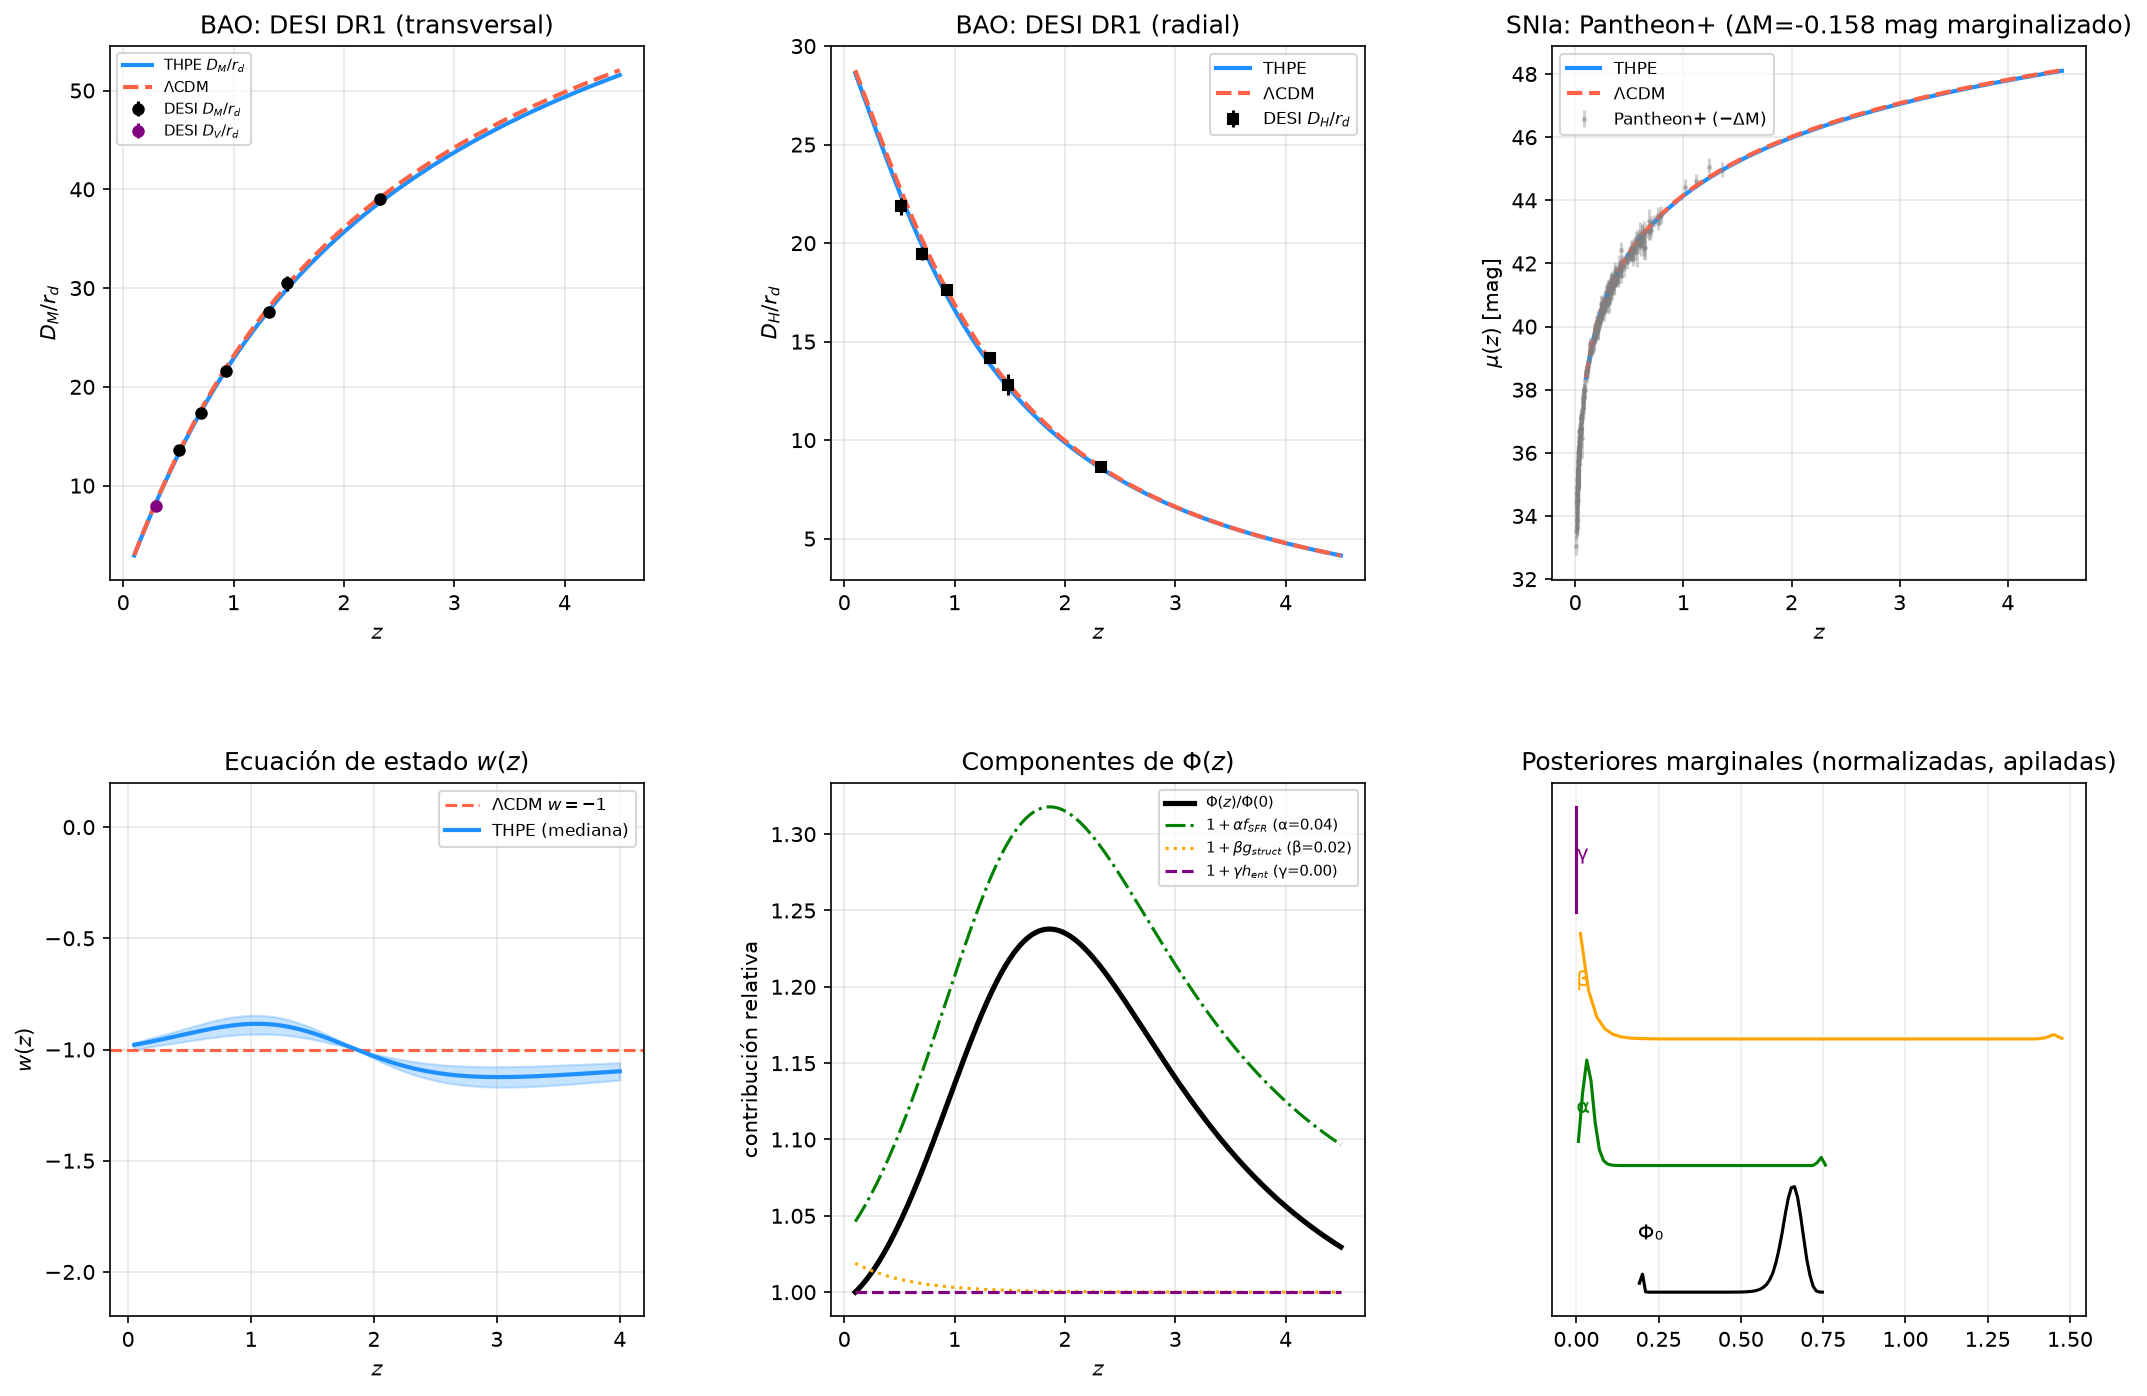
\includegraphics[width=\textwidth]{THPE_v18_dr2_resultados.png}
\caption{Fit of the THPE model to DESI DR2 BAO and Pantheon+ data.
Panels show the transverse and radial BAO observables, the supernova
Hubble diagram with the marginalised magnitude offset applied, the
reconstructed $w(z)$, the individual contributions to $\Phi(z)$, and the
marginal posteriors. The THPE and \LCDM{} curves are indistinguishable
at the resolution of the figure.}
\label{fig:results}
\end{figure*}}{}

\IfFileExists{THPE_v18_dr2_corner.png}{%
\begin{figure}[t]
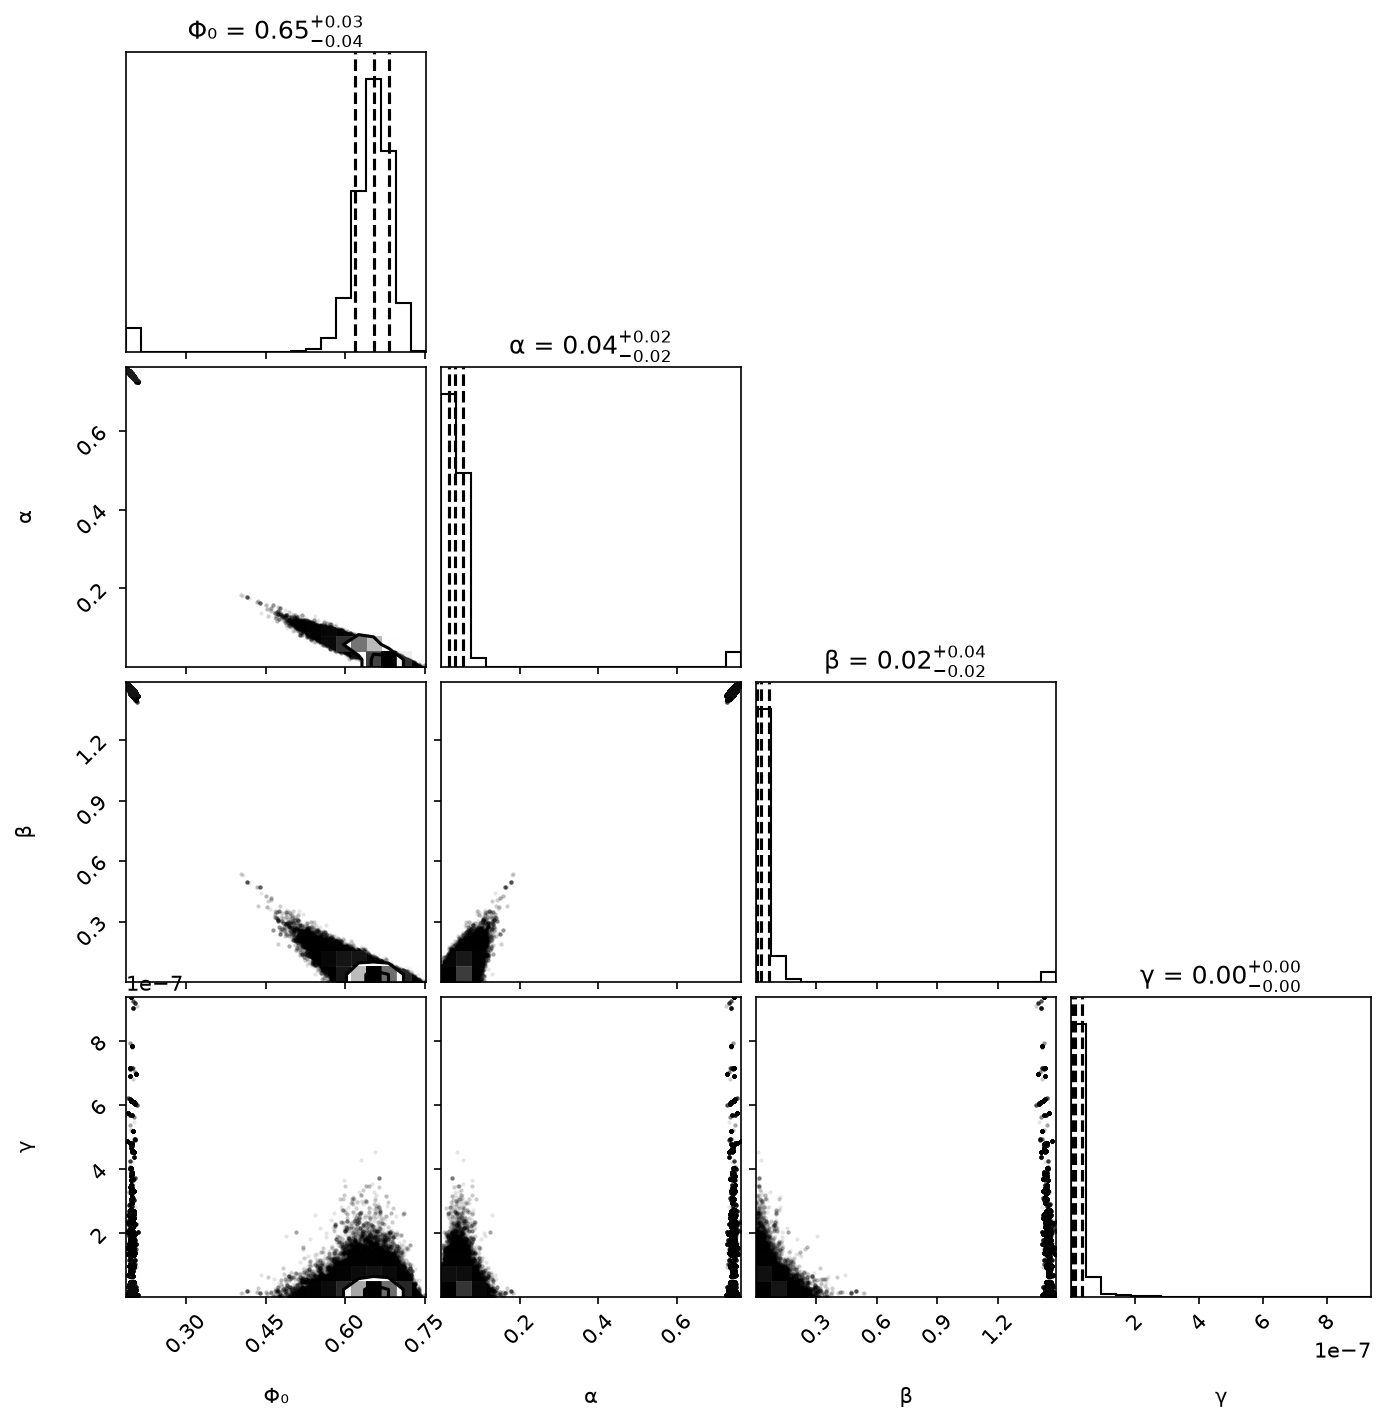
\includegraphics[width=\columnwidth]{THPE_v18_dr2_corner.png}
\caption{Posterior distribution of the four THPE parameters. The
extended $\Phi_0$--$\alpha$--$\beta$ degeneracy is apparent; $\gamma$ is
pinned at zero by the physicality prior.}
\label{fig:corner}
\end{figure}}{}

%=======================================================================
\section{Refutation of the local Compton scale}
\label{sec:compton}
%=======================================================================

An earlier version of the THPE identified the Compton time
$\tau_c=\hbar/Mc^2$ as a universal rate of state compression. Comparing
that scale with experimentally demonstrated quantum coherence times ---
from electron interferometry through molecular interferometry
\cite{Fein2019} to the 40~kg mirrors of LIGO --- the observed coherence
exceeds the prediction by 14 to 51 orders of magnitude across every mass
range ever probed. The identification is therefore refuted.

The only surviving reading of local persistence is strictly relational
(the state $|\psi\rangle$ persists, not a classical trajectory;
compression occurs only through environmental interaction), which is
consistent but operationally equivalent to standard decoherence and thus
carries no additional empirical content. Di\'osi--Penrose-type scales
\cite{Diosi1987,Penrose1996}, $\tau\sim\hbar R/Gm^2$, remain compatible
with all observations and testable with current optomechanics
\cite{Donadi2021}; their exploration lies outside the scope of this
work.

%=======================================================================
\section{Can $\Phi(z)$ be derived?}
\label{sec:derivation}
%=======================================================================

\subsection{Set-up}

We investigated whether Eq.~(\ref{eq:phi}) can be obtained from a
variational principle rather than postulated. The success criterion,
fixed in advance, was to obtain $\Box\Pi=I$ as a \emph{consequence},
with the source $I$ deduced rather than chosen, while passing ghost,
degrees-of-freedom and conservation tests.

\subsection{Minimal case}

Consider the simplest possible non-minimal coupling,
%
\begin{equation}
S=\int d^4x\sqrt{-g}\left[\frac{F(\Pi)R}{2\kappa}
-\frac{\omega}{2}(\partial\Pi)^2-V(\Pi)\right]+S_m,
\label{eq:action}
\end{equation}
%
with $F(\Pi)=1+2\kappa\xi\Pi$. Variation with respect to $\Pi$ gives
%
\begin{equation}
\omega\,\Box\Pi+\xi R-V'(\Pi)=0
\quad\Longrightarrow\quad
\Box\Pi=\frac{V'(\Pi)-\xi R}{\omega}.
\label{eq:boxpi}
\end{equation}
%
The target equation therefore emerges, and the source is \emph{not}
free: $I\propto R$ in vacuum and $I\propto T$ (the trace of the
energy-momment tensor) in the presence of matter, via the trace of the
modified Einstein equations, yielding the canonical Brans--Dicke form
$(2\omega_{\rm BD}+3)\Box\Pi=\kappa T$.

All three consistency tests are passed. In the Einstein frame the
kinetic coefficient is
%
\begin{equation}
K_E=\frac{\omega}{F}+\frac{3}{2\kappa}\left(\frac{F'}{F}\right)^2
=\frac{\omega F+6\kappa\xi^2}{F^2}>0
\quad\text{for }\omega>0,\;F>0,
\label{eq:noghost}
\end{equation}
%
so there is no ghost provided $F>0$ (the region $F<0$ must be excluded
by a physicality prior, in exact analogy with the prior used in the
cosmological analysis). The theory propagates three degrees of freedom
(two tensor, one scalar) with $c_{\rm gw}=c$ exactly, compatible with
GW170817 \cite{GW170817}. Energy--momentum conservation holds
identically because matter couples minimally to $g_{\mu\nu}$ in the
Jordan frame.

\subsection{The bottleneck is local, not cosmological}

The extra scalar mode is precisely that of Brans--Dicke
\cite{BransDicke1961}, with
$\omega_{\rm BD}=\omega F/(F')^2$. The Cassini bound
$\omega_{\rm BD}>4\times10^4$ \cite{Bertotti2003} implies
%
\begin{equation}
|\xi|<2.5\times10^{-3}\kappa^{-1}
\quad\Longrightarrow\quad
\left|\frac{\delta H}{H}\right|<2.5\times10^{-5}.
\label{eq:cassini}
\end{equation}
%
The Solar System limit is thus roughly \emph{400 times more
restrictive} than the cosmological bounds of Eq.~(\ref{eq:bounds}). The
minimal formulation is consistent but indistinguishable from \LCDM{} by
construction --- and would remain so for any future cosmological
dataset.

\subsection{Screening mechanisms}

A field-dependent kinetic term $Z(\Pi)$ cannot produce screening. The
redefinition
%
\begin{equation}
\frac{d\phi}{d\Pi}=\sqrt{Z(\Pi)}
\label{eq:redef}
\end{equation}
%
removes any $Z(\Pi)>0$, returning the theory of
Eq.~(\ref{eq:action}) written in different field-space coordinates; the
effective coupling is $F'/\sqrt{Z}$, a fixed number rather than a
function of the environment. Genuine screening requires dependence on
the local density (chameleon \cite{Khoury2004}, symmetron) or on the
derivatives $X=-(\partial\Pi)^2/2$ (K-mouflage, Vainshtein). The former
are subject to the no-go theorem of Wang, Hui and Khoury
\cite{Wang2012}, which forbids self-acceleration.

\subsection{Vainshtein and Horndeski}
\label{sec:horndeski}

After GW170817, the viable Horndeski Lagrangian reduces to
%
\begin{equation}
\mathcal{L}=G_2(\Pi,X)+G_3(\Pi,X)\Box\Pi+G_4(\Pi)R,
\qquad G_5=0,
\label{eq:horndeski}
\end{equation}
%
and Vainshtein screening \cite{Vainshtein1972} from the $G_3$ term does
resolve Eq.~(\ref{eq:cassini}): the solar Vainshtein radius is
$r_V=(r_s L_c^2)^{1/3}\simeq3.8\times10^{18}$~m $\simeq124$~pc,
suppressing the fifth force by $\sim10^{-9}$ at Neptune's orbit. A
cosmological window between $10^{-3}$ and $10^{-2}$ remains, bounded
above by Eq.~(\ref{eq:bounds}) and further restricted by graviton decay
into dark energy \cite{Creminelli2018} and by gradient-stability
requirements \cite{Kobayashi2019}.

However, the local formulation analysed for $\Pi$ is mathematically
equivalent to a subclass of Galileon/Horndeski theories
\cite{Deffayet2009} within the adopted hypotheses. The retarded
solution of Eq.~(\ref{eq:boxpi}),
%
\begin{equation}
\Pi(x)=\int G_{\rm ret}(x,y)\,I(y)\sqrt{-g}\;d^4y,
\label{eq:retarded}
\end{equation}
%
is a mathematical property of \emph{any} sourced field --- the retarded
Li\'enard--Wiechert potentials have possessed such ``causal memory''
since 1898 --- and adds neither degrees of freedom nor distinctive
predictions.

\subsection{The Planck scale: the real limit of the programme}
\label{sec:planck}

The original intuition placed state persistence at the Planck scale,
$t_P=\sqrt{\hbar G/c^5}\simeq5.4\times10^{-44}$~s, with
$\ell_P=c\,t_P$. Yet the Planck time appears nowhere in the formulation
analysed above: Eq.~(\ref{eq:boxpi}) is a continuous wave equation and
Eq.~(\ref{eq:retarded}) integrates over a continuous past light cone.
Formalising $\Pi$ as a classical field with a covariant action removes
the discreteness by construction.

In this formulation gravity influences $\Pi$ in two ways, neither
involving the Planck scale: as a \emph{source}, through $R$ (and
through $T$ in the presence of matter) in Eq.~(\ref{eq:boxpi}); and as a
\emph{response}, through the $F(\Pi)R$ term, which makes the effective
gravitational constant depend on $\Pi$ and is precisely what
Eq.~(\ref{eq:cassini}) constrains. Both effects are macroscopic and
classical.

This yields a sharper reading of our result: the local formulation does
not fail because of the Cassini bound --- Vainshtein screening resolves
that --- but because, on being made rigorous, it \emph{loses the
ingredient that made it distinctive}. A classical field theory cannot
represent Planck-scale granularity, and without it $\Pi$ is one more
scalar field. If state persistence is genuinely a Planck-scale
phenomenon, its description requires a quantum gravity framework rather
than an effective field theory. We regard this --- rather than the
observational constraints --- as the real limit of the theoretical
programme presented here.

\subsection{Precedent in the literature: Everpresent Lambda}
\label{sec:everpresent}

It is natural to ask whether that route has already been taken. It has.
In causal set theory, Lorentz covariance imposes a Poisson relation
between the spacetime volume of a region and the number $N$ of discrete
elements it contains. From this Sorkin \cite{Sorkin1991,Sorkin2000}
deduced a fluctuating cosmological constant with
$\delta\Lambda\sim1/\sqrt{V}\sim1/\sqrt{N}$: the accumulation of
discrete Planck-scale elements produces, in the macroscopic limit,
dynamical dark energy. The effect is explicitly described as a residual,
non-local quantum consequence of the underlying discreteness
\cite{Ahmed2004,Ahmed2013}. The prediction predates the 1998 discovery
of cosmic acceleration and its order of magnitude agrees with the
observed value without fine-tuning.

The correspondence with the motivation of the present work is close and
we state it explicitly: both start from Planck-scale discrete structure,
both posit that its accumulation affects the expansion, both produce
dynamical dark energy, and both are non-local by construction. The
difference is formal status: Everpresent Lambda \emph{derives} the
fluctuation from a quantum gravity theory, whereas the THPE
\emph{postulated} the functional form of Eq.~(\ref{eq:phi}) from
phenomenological tracers.

That programme is likewise constrained, and by the same observable:
since the everpresent $\Lambda$ originates in past light cones, regions
of the last-scattering surface separated by more than a causal horizon
would carry uncorrelated values, producing CMB anisotropies; the
resulting bound is too small to account for late-time acceleration
\cite{Barrow2007}. The conclusion of Sec.~\ref{sec:horndeski} is
therefore reinforced rather than weakened: the Planck route is not free
territory left unexplored, but ground already covered, formalised and
observationally restricted.

%=======================================================================
\section{Discussion and limitations}
\label{sec:discussion}
%=======================================================================

Three lessons follow. First, the functional form of $\Phi(z)$ is not
what the data require: the DR2--Planck tension projects onto the
amplitude of dark energy rather than its shape. Second, the
$\Phi_0$--$\alpha$--$\beta$ degeneracy is structural; separating the
contributions would require growth observables such as $f\sigma_8$
rather than purely geometric ones. Third, $h_{\rm ent}$ must either be
reformulated from theory, regularising its $z\to0$ divergence, or
dropped.

Limitations are stated explicitly. $H_0$ and $\Omega_m$ are fixed to
Planck values; marginalising over them would broaden the bounds of
Eq.~(\ref{eq:bounds}) without changing the sign of
Eqs.~(\ref{eq:lnB1})--(\ref{eq:lnB2}), which is dominated by the Occam
penalty. We do not use the full CMB likelihood, nor structure growth.
The CMB priors are self-calibrated as described in
Sec.~\ref{sec:data}. The theoretical analysis is restricted to local,
single-field, second-order actions within the space of
Eq.~(\ref{eq:horndeski}); genuinely non-local formulations
\cite{Deser2007}, history functionals, and multi-field sectors are
\emph{not} refuted here --- they were not examined.

%=======================================================================
\section{Conclusions}
\label{sec:conclusions}
%=======================================================================

We have promoted the THPE from proposal to tested hypothesis on two
independent fronts.

Observationally, with the best available public geometric datasets and
explicit validity controls, the evidence strongly favours \LCDM{}
($\ln B$ from $-7.4$ to $-14.8$), excludes the horizon-entropy term, and
bounds informational contributions below $\sim1\%$ of the dark energy
density.

Theoretically, the target equation can be derived from an action
principle, but the resulting local formulation is localised within an
already studied space of theories and provides no independent
phenomenology. The Compton scale is refuted as a physical compression
rate, and the Planck-scale route proves already covered and constrained
in the causal set literature.

The THPE is not falsified: it is \emph{bounded}, and its local
formulation is \emph{closed}. We regard this set of negative results as
a legitimate scientific product: it delimits the viable space of the
hypothesis, documents methodological warnings of general utility (the
non-convergence of ensemble samplers on degenerate posteriors; the
necessity of coherence controls in model comparison), and leaves a
falsifiable prediction with a verifiable time stamp.

%=======================================================================
\section{Future testability}
\label{sec:future}
%=======================================================================

The distinctive prediction of the THPE --- a crossing of $w(z)=-1$ whose
chronology follows the star formation peak at $z\simeq1.9$ --- is
\emph{not} testable at present precision: the permitted couplings,
Eq.~(\ref{eq:bounds}), place the signature below the threshold of
current geometric data.

The datasets that will permit the test are the final DESI release
(expected around 2028--2029, on whatever schedule the collaboration
establishes), the cosmological releases of Euclid \cite{Euclid2011}
(2026--2030), and LSST at the Vera C. Rubin Observatory
\cite{LSST2019} from approximately 2027.

The public, dated registration of this prediction (repository commits of
July 2026) precedes those data. Should dark energy prove dynamical with
the predicted chronology, temporal priority is verifiable; should
$w=-1$ be consolidated at sub-percent precision, the THPE will be
refuted in its reformulations as well, and the authors will say so.

%=======================================================================
\section*{Code and data availability}
%=======================================================================

The complete pipeline, the full correction history and the coherence
controls are publicly available at
\url{https://github.com/moimora1/THPE} (version 1.8):
\texttt{THPE\_fit\_v18.py} (MCMC fit to DESI DR1/DR2 and Pantheon+),
\texttt{THPE\_dynesty\_v1.py} (Bayesian evidence, BAO+SNe) and
\texttt{THPE\_dynesty\_v2\_cmb.py} (evidence with the CMB anchor). The
\texttt{CHANGELOG} documents every version, including the errors
detected and corrected during this work. Pantheon+ data are not
redistributed; the scripts download them from the official
\texttt{PantheonPlusSH0ES/DataRelease} repository.

%=======================================================================
\begin{acknowledgments}
Code development, symbolic and numerical auditing, and technical writing
were assisted by artificial intelligence systems (Claude, Anthropic;
GPT, OpenAI) used with separated roles --- one proposing theoretical
formulations, the other verifying them --- with cross-auditing in both
directions and under human direction throughout. All scientific
decisions and responsibility for the content rest with the human
authors.
\end{acknowledgments}

%=======================================================================
\begin{thebibliography}{99}

\bibitem{DESI2024} DESI Collaboration, \emph{DESI 2024 VI:
Cosmological Constraints from the Measurements of Baryon Acoustic
Oscillations}, arXiv:2404.03002.

\bibitem{DESI2025} DESI Collaboration, \emph{DESI DR2 Results II:
Measurements of Baryon Acoustic Oscillations and Cosmological
Constraints}, arXiv:2503.14738.

\bibitem{Madau2014} P.~Madau and M.~Dickinson,
Annu. Rev. Astron. Astrophys. \textbf{52}, 415 (2014).

\bibitem{Banks2011} T.~Banks and W.~Fischler,
\emph{Holographic Space-Time}, arXiv:1109.2435.

\bibitem{Scolnic2022} D.~Scolnic \emph{et al.},
Astrophys. J. \textbf{938}, 113 (2022).

\bibitem{Planck2020} Planck Collaboration,
Astron. Astrophys. \textbf{641}, A6 (2020).

\bibitem{Chen2019} L.~Chen, Q.-G.~Huang and K.~Wang,
J. Cosmol. Astropart. Phys. \textbf{02}, 028 (2019).

\bibitem{Speagle2020} J.~S.~Speagle,
Mon. Not. R. Astron. Soc. \textbf{493}, 3132 (2020).

\bibitem{emcee} D.~Foreman-Mackey, D.~W.~Hogg, D.~Lang and J.~Goodman,
Publ. Astron. Soc. Pac. \textbf{125}, 306 (2013).

\bibitem{Fein2019} Y.~Y.~Fein \emph{et al.},
Nat. Phys. \textbf{15}, 1242 (2019).

\bibitem{Diosi1987} L.~Di\'osi, Phys. Lett. A \textbf{120}, 377 (1987).

\bibitem{Penrose1996} R.~Penrose,
Gen. Relativ. Gravit. \textbf{28}, 581 (1996).

\bibitem{Donadi2021} S.~Donadi \emph{et al.},
Nat. Phys. \textbf{17}, 74 (2021).

\bibitem{GW170817} B.~P.~Abbott \emph{et al.} (LIGO Scientific
Collaboration, Virgo Collaboration, Fermi-GBM and INTEGRAL),
Astrophys. J. Lett. \textbf{848}, L13 (2017).

\bibitem{BransDicke1961} C.~Brans and R.~H.~Dicke,
Phys. Rev. \textbf{124}, 925 (1961).

\bibitem{Bertotti2003} B.~Bertotti, L.~Iess and P.~Tortora,
Nature \textbf{425}, 374 (2003).

\bibitem{Khoury2004} J.~Khoury and A.~Weltman,
Phys. Rev. Lett. \textbf{93}, 171104 (2004).

\bibitem{Wang2012} J.~Wang, L.~Hui and J.~Khoury,
Phys. Rev. Lett. \textbf{109}, 241301 (2012).

\bibitem{Vainshtein1972} A.~I.~Vainshtein,
Phys. Lett. B \textbf{39}, 393 (1972).

\bibitem{Deffayet2009} C.~Deffayet, G.~Esposito-Far\`ese and A.~Vikman,
Phys. Rev. D \textbf{79}, 084003 (2009).

\bibitem{Creminelli2018} P.~Creminelli, M.~Lewandowski, G.~Tambalo and
F.~Vernizzi, J. Cosmol. Astropart. Phys. \textbf{12}, 025 (2018).

\bibitem{Kobayashi2019} T.~Kobayashi,
Rep. Prog. Phys. \textbf{82}, 086901 (2019).

\bibitem{Deser2007} S.~Deser and R.~P.~Woodard,
Phys. Rev. Lett. \textbf{99}, 111301 (2007).

\bibitem{Sorkin1991} R.~D.~Sorkin, in \emph{Relativity and Gravitation:
Classical and Quantum} (Proc. SILARG VII, Cocoyoc, Mexico, 1990),
World Scientific, p.~150.

\bibitem{Sorkin2000} R.~D.~Sorkin,
Int. J. Theor. Phys. \textbf{39}, 1731 (2000).

\bibitem{Ahmed2004} M.~Ahmed, S.~Dodelson, P.~B.~Greene and
R.~D.~Sorkin, Phys. Rev. D \textbf{69}, 103523 (2004).

\bibitem{Ahmed2013} M.~Ahmed and R.~D.~Sorkin,
Phys. Rev. D \textbf{87}, 063515 (2013).

\bibitem{Barrow2007} J.~D.~Barrow,
Phys. Rev. D \textbf{75}, 067301 (2007);
see also M.~Ahmed \emph{et al.}, arXiv:0711.2904.

\bibitem{Euclid2011} R.~Laureijs \emph{et al.},
\emph{Euclid Definition Study Report}, arXiv:1110.3193.

\bibitem{LSST2019} \v{Z}.~Ivezi\'c \emph{et al.},
Astrophys. J. \textbf{873}, 111 (2019).

\end{thebibliography}

\end{document}
